%version of 07-31-18

\chapter{ARITHMETIC}
\label{ch:arithmetic}

Many, perhaps most, of us take for granted the brilliant notations
that have been developed for the myriad arithmetic constructs that we
use daily.  Our mathematical ancestors have bequeathed us notations
that are not only perspicuous but also convenient for computing and
for discovering and verifying new mathematical truths.  This chapter
is dedicated to sharing this legacy with the reader.

\section{Numbers and Numerals}
\label{sec:numbers-numerals}

\subsection{Introduction}

Every reader will be familiar with the notion of {\it number} and with
the familiar strings, called {\it numerals}, that name numbers.
\index{numbers vs.~numerals}
\begin{quote}
Numbers and numerals embody what is certainly the most familiar
instance of a very important dichotomy that pervades our intellectual
lives: the distinction between objects and their names:

{\em Numbers are intangible, abstract objects.  Numerals are the names
  we use to refer to and manipulate numbers.}

This is a crucially important distinction!  You can ``touch'' a
numeral: break it into pieces, combine two (or more) numerals via a
large range of operations.  Numbers are intangible abstractions: you
cannot compute with them.
\end{quote}
Historically, we have employed a broad range of mechanisms for naming
numbers.

{\Arny I really like the idea of providing some cultural background to
  lure the reader.  I am not sure, however, how much space to
  allocate.  For instance, I like the mention of Roman numerals and of
  the system that the Phoenicians used --- which I am familiar with
  mainly because of Hebrew --- but I am relusctant to go so far as to
  really discuss the formation rules of Roman numerals or the details
  of numeral formation in Hebrew and its kindred languages.}

\noindent
{\it Nicknames for ``popular'' numbers}.
%
At one extreme, we have endowed certain numbers that we are ``fond
of'' with names that do not even hint at the ``meaning of'' the named
number.  To cite just a few examples, we talk about
\begin{itemize}
\item
$\pi$: the ratio of the circumference of a circle to its diameter
\item
$e$: the base of so-called natural logarithms
\item
$\phi$: the {\it golden ratio} (one of several word-names for $\phi$)
  that can be observed in nature, e.g., in the leaf patterns of plants
  such as pineapples and cauliflower
\item
Avogadro's number: a fundamental quantity discussed in chemistry and
physics.  We include this number-name to indicate that not all
special numbers' nicknames are single letters.
\end{itemize}
Nickname-based numerals give no information about the named number:
they do not help anyone (except possibly the {\it cognoscenti:} the
``in-crowd'') {\em identify} the named number, and they do not help
anyone manipulate---e.g., compute with---the named number.  These
names are valuable only for {\em cultural} purposes, not mathematical
ones.

\noindent
{\it Alphabet-based systems.}
%
Several cultures have developed systems for naming arbitrary integers
by using their alphabets in some manner.

One such system that is still visible in European cultures within
constrained contexts comprises so-called {\it Roman numerals}.  One
stills observes these, for instance, as the hour markers on the faces
of ``classical'' clocks and as timestamps on the cornerstones of
offical buildings.  Roman numerals are formed from a constrained set
of letters from the Latin alphabet:

\begin{tabular}{c|c}
{\it Letter} & {\it Numerical value} \\
\hline
I  & 1 \\
V  & 5 \\
X  & 10 \\
L  & 50 \\
C  & 100 \\
D  & 500 \\
M  & 1000
\end{tabular}

\noindent
The formation rules for Roman numerals of length exceeding $2$ are a
bit complicated, but {\em roughly}, a letter to the right of a higher
valued letter augments the value of the numeral (e.g., DCL $=650$, XVI
$=16$), while a letter to the left of a higher valued letter lowers
the value (e.g., MCM $=1900$, XLIV $=44$).

Yet another way to craft numerals from letters is observable in
systems such as is used with the Hebrew alphabet, which incorporates
ideas used by the ancient Egyptians, Phoenicians, and Greeks.  Hebrew
assigns the following respective values to the $22$ letters of its
alphabet.
\[ 1, 2, 3, 4, 5, 6, 7, 8, 9, 10,
20, 30, 40, 50, 60, 70, 80, 90, 100,
 200, 300, 400
\]
Numerals are then formed as strings of single occurrences of letters,
by accumulating the letters' numerical values.  Numbers that are too
large to be named using ``words'' comprising single letter-instances
often allow repeated letter instances or using auxiliary words, in a
mixed-mode manner similar to our writing the number $5000$ as ``$5$
thousand''.


Alphabet-based systems for creating numerals are more useful than
nickname-based systems in that they {\em do} allow anyone to {\em
  identify} any named number.  Indeed, one can (algorithmically)
convert any Roman numeral or any Hebrew numeral to a decimal numeral
for the same number.  However, any reader who is familiar with
alphabet-based systems will recognize a major drawback of such
systems: It is {\em exceedingly difficult} to do any but the most
trivial arithmetic using such systems' numerals.  Two simple examples
using Roman numerals will make our case:
\begin{itemize}
\item
Square CC.  This is, of course, trivial using our familiar decimal
numerals: an elementary school student can compute $200 \times 200 \ =
\ 40,000$.  But even in an early course on programming, one would not
assign the general ``multiply numbers using Roman numerals'' problem
as a first assignment.

\item
Subtract MCMXCVIII from MMII.  We all know, of course, that the answer
is IV, but I had to convert to decimal numerals in order to determine
this.
\end{itemize}

\noindent
{\it Positional number systems.}
%
In our daily commerce, we typically deal with numerals that are formed
within a {\it base-$b$ positional number system,}
\index{numerals in a (base-$b$) positional number system}
%
i.e., by strings of {\it digits} from a set of the form $\{0, 1, 2,
\ldots, \overline{b-1}\}$, often embellished with other symbols, such as
a {\em radix point},\footnote{The use of a period as the radix point
  is a US convention; in much of Europe, a comma usually denotes the
  radix point.}~and sometimes a leading ``$+$'' or ``$-$'' to
indicate, respectively, the denoted number's positivity or negativity.
\begin{quote}
{\em We employ the notation ``$\overline{b-1}$'' to remind ourselves
  that in this context ``$b-1$'' is a digit, not a string; for
  instance, when $b = 10$ (the common {\em decimal} base),
  $\overline{b-1}$ is the digit $9$.  }
\end{quote}
We discuss positional number systems in detail in
Section~\ref{sec:Numerals}.  For now, we settle for a few examples:
\begin{itemize}
\item
Most of our daily work employs the base-$10$ ({\it decimal}) system,
whose digits comprise the set $\{0, 1, 2, 3, 4, 5., 6, 7, 8, 9\}$; the
system's radix point is usually called a {\em decimal point}.

\item
Because electrical and electronic circuitry are (for the most part)
built using {\it bistable} devices---e.g., switches that are either
{\em on} or {\em off}---the system most often employed when dealing
with such circuitry and its end products (say, computers) is the
base-$2$ ({\it binary}) system, whose digits---usually called {\it
  bits}---comprise the set $\{0, 1\}$.

\item
Because of its small repertoire of digits, the binary system's
numerals are quite long---roughly $3$ times longer than decimal
numerals.  For instance,
\[ 32,768 \ \mbox{ base $10$} \ \ = \ 1,000,000,000,000,000 \ \mbox{
  base $2$}
\]
In order to make these numerals easier for humans to deal with, small
sequences of bits are often aggregated to form larger number bases---but
still powers of $2$.  Two aggregations have been particularly popular:
  \begin{itemize}
  \item
By aggregating length-$3$ sequences of bits, one converts binary
numerals to base-$8$ ({\it octal}) numerals; the octal digits comprise
the set $\{0, 1, 3, 4, 5, 6, 7\}$.
  \item
By aggregating length-$4$ sequences of bits, one converts binary
numerals to base-$16$ ({\it hexadecimal}) numerals; the hexadecimal
digits comprise the set
\[ \{0, 1, 3, 4, 5, 6, 7, 8, 9, \overline{10}, \overline{11},
\overline{12}, \overline{13}, \overline{14}, \overline{15}\}.
\]
{\it Note:} We have written the hexadecimal digits in decimal, to make
them easy to read, but we have placed overlines above the $2$-digit
(decimal) numerals ``$10$'', ``$11$'', ``$12$'', ``$13$'', ``$14$'',
and ``$15$'' as a reminder that each represents a single hexadecimal
digit, not a $2$-digit numeral.
  \end{itemize}
\end{itemize}


\subsection{A Brief Biography of Our Number System}
\label{sec:number-taxonomy}
\index{number system!biography}

We begin our study of arithmetic with a short taxonomy of {\it
  numbers}, the objects that arithmetic was invented to explicate and
exploit.  Although we assume that the reader is familiar with the most
common classes of numbers, we do spend some time highlighting
important features of each class, partly, at least, in the hope of
heightening the reader's interest in this most basic object of
mathematical discourse.

We present the four most common classes of numbers in what is almost
certainly the chronological order of their discovery/invention.
\begin{quote}
{\em Did humans {\em invent} these classes of numbers to fill specific
  needs, or did we just {\em discover} their pre-existing selves as
  needs prompted us to search for them?  The great German
  mathematician Leopold Kronecker,
\index{Kronecker, Leopold}
as cited in \cite{Bell86} (page 477), shared his viewpoint on this
question:} ``God made the integers; all else is the work of man.''
\end{quote}
A pleasing narrative can be fabricated to account for our multi-class
system of numbers.  In the beginning, the story goes, we needed to
count things (sheep, bottles of oil, weapons, \ldots), and the
positive {\it integers}\index{number!integer} were discovered to serve
this need.  As accounting practices matured, we needed to augment this
class with the number zero
\index{number!zero ($0$)}
($0$), to allow merchant $A$ to keep track of the remining inventory
after selling the last flask of wine, and with the negative integers,
\index{number!negative}
to allow the  merchant's banker to record $A$'s credit balance after
taking a loan.  The class of integers was now complete, even though
a variety of special classes of integers that warranted special
attention for reasons ranging from the religious to the intellectual
remained to be discovered.  As society matured, humans began to share
materials that had to be be subdivided---cloth, grain, etc.---rather
than partitioned in discrete units.   We needed to invent the {\it
rational numbers}
\index{number!rational}
%
to deal with such materials.  Happily for the mathematically inclined,
the rational numbers could be developed in a way that allowed one to
view an integer as a special type of rational.  This meant that our
ancestors could build upon the systems they had developed to deal with
integers, rather than scrapping those systems and starting anew.
\begin{quote}
{\em This quest for {\em extendible} frameworks rather than isolated
  unrelated frameworks is a hallmark of mathematical thinking.}
\end{quote}
We now enter the realm of ``semi-recorded'' history in the West: the
Babylonians, the Egyptians, the Greeks, and others.  ``Practical''
mathematics was invented---and reinvented---to accommodate pursuits as
varied as astronomy and architecture.  Our mathematical stalwarts, the
integers and the rationals, did not seem to be able to deal with
measurements we wanted to make, calculations we wanted to do,
structures we wanted to design.  So, we approximated and ``fudged''
and got prety much where we wanted to get.  The standard story at this
point (at least in the West) is that the ancient Greeks began to try
to systematize mathematical knowledge and practice.  The Greek
mathematician and geometer Euclid
\index{Euclid}
%
and members of his school verified---via one of the first {\em proofs}
in recorded history---the uncomfortable fact that the lengths of
portions of eminently buildable structures were not ``measurable,'' by
which they meant ``not rational.''  The poster child for this
phenomenon was the hypotenuse of the isosceles right triangle $T$ with
unit-length legs.  {\em There was---provably!---no way to find
  integers $p$ and $q$ whose ratio was the length of $T$'s
  hypotenuse.}\footnote{We describe Euclid's proof in
  Proposition~\ref{thm:sqrt(2)}.}  As part of this same movement
toward formal mathematics, the Sicilian-based Greek mathematician and
polymath Archimedes
\index{Archimedes}
%
was observing that squares are better approximations to circles than
triangles are; regular pentagons are better than squares; regular
hexagons are better than pentagons; and so on.  In fact, as the number
of sides, $n$ in a regular polygon grows without bound (or, as we
might say today, tends to infinity), the regular polygons get closer
and closer to a circle.  
  **HERE
As a response to this discomfort, the
{\it real numbers}\index{number!real} were invented.  Once again,
happily, one could develop the real numbers in a way that allowed one
to view a rational number as a special type of real number.  Time went
on, and mathematics matured.  Polynomials\index{polynomial} and their
roots\index{polynomial!root}\footnote{A number $r$ is a {\it root} of
  a polynomial $P(x)$ if $P(r) =0$.}~were discovered, together with
the next source of discomfort.  To understand this discomfort, one
must note that, since the invention of the real numbers, every
polynomial $P_m(x)\ \eqdef \ x^2 - m$, where $m$ is a nonnegative real
number, had two roots, denoted, respectively, $+\sqrt{m}$ and
$-\sqrt{m}$.  But---here is the source of discomfort---{\em the
  polynomial $P_m(x)$ had no roots when $m$ was negative, even a
  negative \underline{integer}}.  The response this time resided in
the invention of a new {\it imaginary} number,\index{number!imaginary}
called $i$,\index{imaginary number $i = \sqrt{-1}$} that was a root of
the polynomial $P_{-1}(x) = x^2 +1$; $i$ was often defined via the
equation, $i = \sqrt{-1}$; easily, $-i$ is also a root of
$P_{-1}(x)$.  By combining the imaginary number $i$ with the real
number system, the {\it complex numbers}\index{number!complex} were
born.

The reader is possibly anticipating a new ``discomfort'' leading to an
new augmentation of our number system, but, no, the story is now
complete, in the sense expressed in the {\it Fundamental Theorem of
  Algebra}\index{Fundamental Theorem of Algebra}, which asserts:

\begin{theorem}[{\bf The Fundamental Theorem of Algebra}]
\label{thm:fund-thm-algebra}
Every polynomial of degree $n$ with complex coefficients has $n$ roots
over the complex numbers.
\end{theorem}

We return to the later to the Theorem and its applications and
implications.  For now, though, it completes our historical tour, so
we can finally begin to get acquainted with our four classes of
numbers.


\section{Integers}
\label{sec:integers}

The most basic class of numbers are the {\it integers}
\index{number!integer}
(or, {\it whole numbers},
\index{number!integer!whole number}
or, {\em counting numbers}).
\index{number!integer!counting number}
%
Integers are certainly the numbers that our prehistoric ancestors
employed in the earliest days of our species.

\subsection{The Basic of Integers: The Number Line}
\label{sec:number-line}
\index{number!the number line}
\index{number!integer!the number line}
%
We survey a number of the most important properties of the set
$\Z$\index{$\Z$: the set of all integers} that comprises {\em all
  integers} (the positive and negative integers and zero ($0$)) and
the set $\N$\index{$\N$: the set of nonnegative integers} that
comprises the {\em nonnegative integers} (the positive integers and
$0$).  We estimate a property's importance from the vantage points of
both mathematics and its manifold applications.

Several essential properties of $\N$ and $\Z$ are consequences of the
sets' behavior under their natural order relations: strong ($<$) and
weak ($\leq$) and their converses.  Indeed, order within a number
system is one of one's biggest friends when reasoning about the
numbers within the system.
\index{number!ordering of numbers}
\begin{itemize}
\item
The set $\Z$ is {\em totally ordered}\index{number!integer!total
  order}\index{integer!total order}, also termed {\em linearly
  ordered}\index{number!integer!linear ordering}\index{integer!linear
  ordering}.

\smallskip

This fact is embodied in the {\em Trichotomy Laws for
  integers}.\index{number!integer!Trichotomy Laws}
\index{integer!Trichotomy Laws}\index{Trichotomy Laws}

\medskip

{\it The Trichotomy laws for integers}. \\
%
(a)
%
{\it For each integer $a \in \Z$, precisely one of the following is true.}
\[
(1) \ \mbox{ $a$ equals $0$:} \ a=0 \ \ \ \
(2) \ \mbox{ $a$ is {\em positive}:} \ a>0 \ \ \ \
(3) \ \mbox{ $a$ is {\em negative}:} \ a<0
\]

Consequently, $\Z$ can be visualized via the ($2$-way infinite) number
line:
\index{number!the number line}
\[ \ldots, -2, -1, 0, 1, 2, \ldots
\]
Analogously, $\N$ can be visualized via the ($1$-way infinite) number
line: $0, 1, 2, \ldots$.

\medskip

(b)
%
{\it For any integers $a, b \in \Z$, precisely one of the following is
  true.}
\[ (1) \ a=b \ \ \ \ \ \ \ (2) \ a<b \ \ \ \ \ \ \ (3) \ a>b \]

\item
The set $\N$ is {\it well-ordered}.
\index{number!nonnegative integers!well-ordering}
\index{nonnegative!integers!well-ordering}

\medskip

{\it The Well-ordering law for nonnegative integers}. \\
%
{\it Every subset of $\N$ has a smallest element (under the ordering
  $<$).}

\medskip

\item
The set $\Z$ is {\it discrete}.
\index{number!integer!discreteness}\index{integer!discreteness}

\medskip

{\it The discreteness of the integers.} \\
%
{\it For every integer $a \in \Z$, there is no integer between $a$ and
  $a+1$; i.e., there is no $b \in \Z$ such that $a < b < a+1$.}

\medskip

\item
The set $\Z$ obeys the {\it ``Between'' Laws}
\index{number!integer!''Between'' laws}\index{integer!''Between'' laws}

\medskip

{\it The ``Between'' laws for integers}. \\
%
{\it For any integers $a, b \in \Z$, there are finitely many $c \in
  \Z$ such that $a < c < b$.}

\smallskip

Any such $c \in \Z$ is {\em between} $a$ and $b$, whence the name of
the law.
\end{itemize}

\subsection{Prime numbers: building blocks of the integers}
\label{sec:primes}
\index{number!prime numbers}
\index{integers!prime numbers}

We single out a subclass of the positive integers whose mathematical
importance has been recognized for millennia but which have found
important applications (e.g., within the domain of computer security)
mainly within the past several decades.

We say that a positive integer $p$ {\it divides} a positive integer
$n$ (or, {\it is a divisor of $n$})\index{number!integer!divisor} if
there is a positive integer $q$ such that $n = p \cdot q$.
Equivalently, we say that $n$ {\it is divisible
  by}\index{number!integer!divisibility} $p$.  Thus, every positive
integer $n$ is divisible by $p=1$ (witnessed by $q=n$) and by $p=n$
(witnessed by $q=1$).

The class of integers we single out is defined by its divisibility
characteristics.

An integer $p >1$ is {\it prime}\index{number!integer!prime
  number}\index{number!integer!prime}\index{prime
  number}\index{integer!prime number}\index{integer!prime}
if its {\em only} positive integer divisors are $1$ (which divides
every integer) and itself (which is always a divisor).
\begin{quote}
We usually use the shorthand assertion, ``$p$ is a prime,'' instead of
the longer, but equivalent, ``$p$ is a prime integer.''
\end{quote}

\subsubsection{Primes as building blocks: The Fundamental Theorem of Arithmetic}
\label{sec:prime-factoriation}


A very important way to classify a positive integer $n$ is to list the
primes that divide it, coupling each such prime $p$ with its {\it
  multiplicity}, i.e., the number of times that $p$ divides $n$.  Let
$p_1, p_2, \ldots, p_r$ be all of the distinct primes that divide $n$,
and let each $p_i$ divide $n$ with multiplicity $m_i$.  The {\it prime
  factorization}
\index{prime factorization}
\index{integer!prime factorization}
\index{number!integer!prime factorization}
%
of $n$ is the product $p_1^{m_1} \cdot p_2^{m_2} \cdot \cdots \cdot
p_r^{m_r}$; note that this product satisfies the equation
\begin{equation}
\label{eq:prime-factorization}
n \ = \ p_1^{m_1} \cdot p_2^{m_2} \cdot \cdots \cdot p_r^{m_r}
\end{equation}

When writing an integer $n$'s prime factorization, it is traditional
to write the factorization in {\it canonical form},
\index{prime factorization!canonical form}
\index{integer!prime factorization!canonical form}
\index{number!integer!prime factorization!canonical form}
i.e., with the primes $p_1, p_2, \ldots, p_r$ that divide $n$ listed
in increasing order, i.e., so that $p_1 < p_2 < \cdots < p_r$.

\noindent
A positive integer $n$ is totally characterized by its canonical prime
factorization, as attested to by the following classical theorem,
which has been known for millennia and has been honored with the title
{\em The Fundamental Theorem of Arithmetic}.
\index{Fundamental Theorem of Arithmetic}
We state the Theorem in two equivalent ways which suggest different
ways of thinking about the result.

\begin{theorem}[The Fundamental Theorem of Arithmetic]
\index{Fundamental Theorem of Arithmetic}
\label{thm:Fund-Thm-Arith}

\noindent
{\rm (Traditional formulation.)}
%
The canonical prime factorization of every positive integer is unique.

\noindent
{\rm (Alternative formulation.)}
%
Let $n \in \N^+$ be a positive integer, and let $\widehat{P}_n$ denote the
ordered sequence of prime numbers that are no larger than $n$:

\begin{tabular}{ll}
$\widehat{P}_n \ =$  & $\langle P_1, \ P_3, \ \ldots, \ P_{r-1}, \ P_r \rangle$ \\
where:               & $P_1 \ = \ 2$ \\
                     & each  \ \ $P_i \ < \ P_{i+1}$ \\
                     & $P_r \ \leq \ n$.
\end{tabular}

\noindent
There exists a unique sequence of {\em nonnegative} integers, 
$\langle a_1, a_2, \ldots, a_r \rangle$
such that
\[
n \ = \ \prod_{i=1}^r \ P_i^{a_i} \ = \
P_1^{a_1} \cdot P_2^{a_2} \cdot \ \cdots \ \cdot P_{r-1}^{a_{r-1}} \cdot P_r^{a_r}
\]
\end{theorem}

A simple, yet important, corollary of Theorem~\ref{thm:Fund-Thm-Arith}
is the following result, whose proof we leave to the reader.

\begin{prop}
\label{thm:prime-divisor}
Every positive integer is divisible by at least one prime number.
\end{prop}


\subsubsection{Proving the Fundamental Theorem of Arithmetic}

The  proof of Theorem~\ref{thm:Fund-Thm-Arith} is actually rather
elementary, providing that one approaches it gradually.  It
employs a lot of important techniques and concepts involved in ``doing
mathematics'', as discussed in the eponymous Chapter~\ref{ch:doingmath}.

We begin with a purely technical result.

\begin{prop}
\label{thm:p-n-linear}
Let $p$ be a prime, and let $m$ be any positive integer that is {\em
  not} divisible by $p$.  There exist integers $a, b$, not necessarily
positive, such that
\[ ap + bm \ = \ 1. \]
\end{prop}

\begin{proof}
Consider the set of all integer linear combinations of $p$ and $m$:
\[  L_{p,m} \ \eqdef \   \{ ap +bm \ | \ a, b \in \Z \} \ \subseteq \ \Z. \]
Note that both $p$ and $m$ belong to $L_{p,m}$, because of the
respective cases $(a=1, b=0)$ and $(a=0, b=1)$.  One consequence of
this is that $L_{p,m}$ has a nonempty subset, call it
$L^{(>0)}_{p,m}$, all of whose elements are {\em positive} integers.

By the {\it Well-Ordering Principle of the positive integers}, the set
$L^{(>0)}_{p,m}$ has a smallest element, call it $r_0$.  By definition
of $L^{(>0)}_{p,m}$, $r_0$ is a positive integer, and there exist
integers $a_0$ and $b_0$ such that
\[  r_0 \ = \ a_0 p + b_0 m. \]

We claim that $L^{(>0)}_{p,m}$ in fact {\em consists precisely of all
  positive-integer multiples of $r_0$.}  Were this not the case, there
would be an element $r$ of $L^{(>0)}_{p,m}$ that is not a
(positive-integer) multiple of $r_0$.  Let $r_1$ be the {\em smallest}
such element $r$.  We then have
\begin{enumerate}
\item
Because $r_1 \in L^{(>0)}_{p,m}$, there exist integers $a_1$ and $b_1$
such that
\[  r_1 \ = \ a_1 p + b_1 m. \]
\item
Because $r_0$ is the {\em smallest} element of $L^{(>0)}_{p,m}$, we
have $r_2 \ \eqdef \ r_1 - r_0 \ > 0$, so that
\[ r_2 \ = \ (a_1 - a_0) p + (b_1 -b_0) m \ \in \ L^{(>0)}_{p,m}. \]
\end{enumerate}
Now, we are in trouble because of the following incompatible facts.
\begin{itemize}
\item
$r_2$ {\em is not} a multiple of $r_0$!

If it were, then we would have $r_0$ dividing both $r_0$ (trivially)
and $r_2 = r_1 - r_0$.  But this would imply that $r_0$ divides $r_1$,
contrary to assumption.

\item
$r_2$ {\em is} a multiple of $r_0$!

This is because $r_2 < r_1$, and $r_1$ is the {\em smallest} element
of $L^{(>0)}_{p,m}$ that is not a multiple of $r_0$.
\end{itemize}
We conclude that integer $r_1$ does not exist, so that all elements of
$L^{(>0)}_{p,m}$ are multiples of $r_0$.

Let us summarize.  The set of positive integer linear combinations of
$p$ and $m$ consists of the multiples of a single integer $r_0$.  This
means, in particular, that both $p$ and $m$ are multiples of a single
positive integer, $r_0$---even though $p$ is a prime which does not
divide $m$.  The only way this situation could hold is if $r_0 = 1$,
as claimed in the proposition.  \qed
\end{proof}

\begin{prop}
\label{thm:p-divides-onefactor}
If the prime $p$ divides a composite number $m \cdot n$, then either
$p$ divides $m$, or $p$ divides $n$, or both.\footnote{The closing
  phease ``or both'' signals our use of the {\em inclusive} or.}
\end{prop}

\begin{proof}
Let $p$, $m$, and $n$ be as asserted, and say that $p$ does not divide
$m$.  By Proposition~\ref{thm:p-n-linear}, then, there exist integers
$a, b$, not necessarily positive, such that
\[ ap + bm \ = \ 1. \]
Let us multiply both sides of this equation by $n$.  After some
manipulation---specfically, applying the distributive law---we find
that
\[ apn + bmn \ = \ n. \]
Now $p$ divides the expression to the left of the equal sign: $p$
divides $p$ by definition, and $p$ divides $mn$ by assumption.  It
follows that $p$ must divide the expression to the right of the equal
sign---namely, the integer $n$.  \qed
\end{proof}

We are finally ready to develop the proof of the Fundamental Theorem.

%\addcontentsline{toc}{paragraph}{Proof of the Fundamental Theorem of Arithmetic}

\begin{proof}
{\bf Proof of the Fundamental Theorem of Arithmetic.}
%
Our dominant tool for proving Theorem~\ref{thm:Fund-Thm-Arith} will be
{\em proof by contradiction} (see Chapter~\ref{sec:Contradiction}).
We assume, for the sake of contradiction, that there is a positive
integer $n$ that has two distinct canonical prime factorizations.

Our argument will be a trifle simpler if we employ the {\em alternative} 
form of the Theorem.  To this end, let
\[ P_1 \ < \ P_2 \ < \cdots < \ P_{r-1} \ < \ P_r \]
denote, in increasing order, the set of all primes that do not exceed
$n$; i.e., every $P_i \leq n$.

The fact that $n$ has two distinct canonical prime factorizations
manifests itself, in this formulation, by the assumption that there
exist {\em two} distinct sequences of {\em nonnegative} integers, 
\[ \langle a_1, a_2, \ldots, a_r \rangle \ \ \ \mbox{ and } \ \ \
\langle b_1, b_2, \ldots, b_r \rangle 
\]
such that $n$ is expressible by---i.e., is equal to---both of the
following products of the primes $P_1$, $P_2$, \ldots, $P_{r-1}$, $P_r$.
\begin{eqnarray}
 & & 
\label{eq:product1.1}
P_1^{a_1} \cdot P_2^{a_2} \cdot \ \cdots \ \cdot P_{r-1}^{a_{r-1}}
\cdot P_r^{a_r} \\
 & &
\label{eq:product2.1}
P_1^{b_1} \cdot P_2^{b_2} \cdot \ \cdots \ \cdot P_{r-1}^{b_{r-1}}
\cdot P_r^{b_r}
\end{eqnarray}

Let us now ``cancel'' from the products (\ref{eq:product1.1}) and
(\ref{eq:product2.1}) the longest common prefix.  Because the two
products are, by hypothesis, distinct, at least one of them will not
be reduced to $1$ by this cancellation.  We are, therefore, left with
residual products of the forms
\begin{eqnarray}
 & &
\label{eq:product1.2}
P_i^{a_i} \cdot X \\
 & &
\label{eq:product2.2}
P_i^{b_i} \cdot Y
\end{eqnarray}
where:
\begin{itemize}
\item
Precisely one of $a_i$ and $b_i$ equals $0$.

Say, with no loss of generality (because we have no intrinsic way to
distinguish the products), that $b_i =0$ while $a_i \neq 0$.

\item
Products $X$ and $Y$ are composed only of primes that are strictly
bigger than $P_i$.
\end{itemize}
Note that 
\[ P_i^{a_i} \cdot X \ = \ P_i^{b_i} \cdot Y \ = \ Y, \]
because these products result from cancelling the same prefix from the
equal products (\ref{eq:product1.1}) and (\ref{eq:product2.1}), and
because $b_i =0$ so that $P_i^{b_i} = 1$.

We have finally reached the point of contradiction.

On the one hand, $P_i$ {\em must} divide the product $Y$, because it
divides the product $P_i^{a_i} \cdot X$ which equals $Y$.

On the other hand, $P_i$ {\em cannot} divide the product $Y$, because
every prime factor of $Y$ is bigger than $P_i$ (and a prime cannot
divide a bigger prime).

We conclude that one of the products (\ref{eq:product1.1}) and
(\ref{eq:product2.1}) cannot exist, so the theorem must hold.  \qed
\end{proof}



\subsubsection{A technical application of the Theorem: There are
  infinitely many primes}
\label{sec:infinite-primes}

The following result, which is traditionally attributed to the Greek
mathematician Euclid, \index{Euclid} one of the patriarchs of
mathematics, invokes Theorem~\ref{thm:Fund-Thm-Arith} in a crucial
way.

\begin{prop}
\label{thm:infinite-primes}
There are infinitely many prime numbers.
\end{prop}

\begin{proof}
Let us assume, for the sake of contradiction, that there are only
finitely many primes.  Say, in particular, that the following
$r$-element sequence enumerates all (and only) primes, in order of
magnitude:

\noindent
$\mbox{\bf Prime-Numbers} \ = \ 
\langle P_1, \ P_2, \ \ldots, \ P_r \rangle$

\noindent where
\[ P_1 \ < \ P_2 \ < \cdots < \ P_{r-1} \ < \ P_r \]
Of course, we know that the first several primes are
\[ (P_1 =2), \ (P_2 = 3), \ (P_3 =5), \ (P_4 = 7), \ (P_5 =11), \ldots \] 

We verify the {\em falseness} of the alleged completeness of the sequence
{\bf Prime-Numbers} by analyzing the positive integer
\[ n \ = \ 1 + \prod_{i=1}^r \ P_i \ = \ 1 \ + \ 
\left(P_1 \cdot P_2 \cdot \cdots \cdot P_r \right).
\]

We make three crucial observations.

\begin{enumerate}
\item
We note first that {\em the number $n$ is not divisible by any prime
number  in the sequence {\bf Prime-Numbers}.}

To see this, note that for each $P_k$ in the sequence,
\[
n / P_k \ = \ \frac{1}{P_k} \ + \ \prod_{i \neq k} \ P_i .
\]
Because $P_k \geq 2$, we see that $n / P_k$ obeys the inequalities
\[
\prod_{i \neq k} \ P_i \ < \ n/P_k \ < \ 1 + \prod_{i \neq k} \ P_i.
\] 
The discreteness of the set $\Z$---see
Section~\ref{sec:number-line}---implies that $n / P_k$ is not an
integer, because it lies strictly between two adjacent integers.

\item
We note next that, because of assertion 1, if the sequence {\bf
  Prime-Numbers} actually did contain {\em all} of the prime numbers,
then we would have to conclude that {\em the number $n$ is not
  divisible by any prime number.}

\item
Finally, we remark that the Fundamental Theorem of Arithmetic
(Theorem~\ref{thm:Fund-Thm-Arith}) implies that {\em every integer is
  divisible by (at least one) prime number}.
\end{enumerate}
The preceding chain of assertions leads to a mutual inconsistency.  On
the one hand, the integer $n$ has no prime-integer divisor.  On the
other hand, no integer can fail to have a prime-integer divisor!

Let us analyze how we arrived at this uncomfortable place.
\begin{itemize}
\item
At the front end of this uncomfortable string of assertions we have
the assumption that there are only finitely many prime numbers.  We
have (as yet) no substantiation for this assertion.
\item
At the back end of this uncomfortable string of assertions, we have
the ({\em rock solid}) Fundamental Theorem of Arithmetic
(Theorem~\ref{thm:Fund-Thm-Arith}).
\item
In between these two assertions we have a sequence of assertions, each
of which follows from its predecessors via irrefutable rules of
inference.
\end{itemize}
It follows that the {\em only} brick in this edifice that could be
faulty---i.e., the only assertion that could be false---is the initial
assumption, which states that there are only finitely many prime
numbers.  We must, therefore, conclude that this vulnerable assumption
is false!  In other words, we conclude from this classical proof by
contradiction that there are infinitely many prime numbers.  \qed
\end{proof}


\subsubsection{Applying the Theorem in {\em encryption}}
\label{sec:Primes-and-encryption}

One of the most important applications of Theorem~\ref{thm:Fund-Thm-Arith} is
as a mechanism for facilitating {\em encryption}.
\index{number!using the Fundamental Theorem of Arithmetic for encoding}
\index{number!using prime numbers for encoding}
\index{encoding sequences via the Fundamental Theorem of Arithmetic}
%
While the details of both encryption and the use of prime numbers to
that end are beyond the scope of this text, we will provide a peek
into that area by means of the following result concerning {\it
  encodings}.
\begin{quote}
{\em 
There is a crucial difference between {\em encoding} and {\em
  encryption}, despite the words' often being confused in the
vernacular.

Encoding involves a search for representations of objects, to achieve
some benefit, such as efficient computation or compactness.  An
example might be the conversion of Roman numerals to positional
numerals to enhance the arithmetic operations.

Encryption usually has some notion of secrecy attached.  An example
might be some key-based cipher which is intended to limit access to
someinformation.  }
\end{quote}


sequences of positive integers as single integers!  This works as
follows.  Consider the (infinite) ordered sequence of {\em all primes:}
\[ (P_1 = 2), (P_2 = 3), (P_3 = 5), \ldots  \]
Let
\begin{equation}
\label{eq:sequence-vec-s}
\bar{s} \ = \ \langle m_1, m_2, \ldots, m_k \rangle
\end{equation}
be an arbitrary sequence of positive integers.  Then
Theorem~\ref{thm:Fund-Thm-Arith} assures us that the (single) positive
integer
\[ 
\iota(\bar{s}) \ \eqdef \ P_1^{m_1} \cdot P_2^{m_2} \cdot \ \cdots \
\cdot P_k^{m_k}
\]
is a (uniquely decodable) integer-representation of sequence $\bar{s}$.

We return to this idea of encoding-via-integers in a later chapter.

\subsubsection{{\bf Enrichment}: The ``density'' of the prime numbers}
\label{sec:Prime-Number-Theorem}

{\Arny There are two advanced topics that we may want to
  mention/discuss: (1) The prime-number theorem ($n/ \log n$ primes
  $\leq n$); (2) the polynomials that generate lots of primes.  We
  should discuss this}


\section{The Rational Numbers}
\label{sec:rationals}

\subsection{Inventing the Rational Numbers}

Each augmentation of our number system throughout history has been a
response to a deficiency with the then-current system.  The deficiency
that instigated the introduction of the rational numbers was the
frequency with which a given integer $q$ does not divide another given
integer $p$.  This fact meant that the operation of multiplication
could often not be ``undone'', or ``inverted'', because division, the
operation that would accomplish the undoing/inverting, would be a {\em
  partial operation:} There are pairs of integers neither of which
divides the other.  The defining characteristic of the expanded system
is that, within it, every nonzero number divides every number.


\subsection{The Rationals as Ordered Pairs of Integers}

The set $\Q$ of {\it rational} numbers\index{number!rational}
\index{$\Q$: the set of rational numbers}
consists of the number $0$, plus the ratios $p/q$ of all nonzero
integers:
\[ \Q \ \eqdef \ \{0\} \ \cup \ \left\{ p/q \ | \ p, q \in \Z
\setminus \{0\} \right\}
\]
Each element of $\Q$ is called a {\it rational} number;
\index{number!rational} 
each {\em nonzero} rational number $p/q$ is often called a {\em
  fraction},
\index{number!fraction}
especially when $q > p$.

An alternative, mathematically more advanced, way of defining the set
$\Q$ is to view it as the smallest set of numbers that contains the
integers, i.e., the set $\Z$, and is {\it closed under the operation
  of dividing any number by any nonzero number.}
\index{algebraic closure}
The word ``closed'' here means that, given any two numbers in $\Q$,
call them $r$ and $s \neq 0$, their quotient $r/s$ belongs to $\Q$.

Numerous notations have been developed for ``naming'' rational numbers
in terms of the integers they are ``built from.''  Most of these
notations continue our custom of employing the symbol ``$0$'' for the
number $0$.  For the nonzero elements of $\Q$, we traditionally employ
some notation for the operation of division and denote the
\begin{equation}
\label{eq:fraction}
 p/q \ \ \ \mbox{ or } \ \ \ {p \over q} \ \ \ \mbox{ or } \ \ \ p
 \div q
\end{equation}
The integer $p$ in any of the expressions in (\ref{eq:fraction}) is
the {\it numerator}
\index{number!rational!numerator}
\index{number!fraction!numerator}
of the fraction; the integer $q$ is the {\it denominator}.
\index{number!rational!denominator}
\index{number!fractions!denominator}


\subsection{Comparing the rationals with the integers}

There are many ways to compare the sets $\Z$ and $\Q$ via properties
that enhance our understanding of the two sets.

\medskip

{\it i. Every integer is a rational.}
%
Obviously, every integer $n \in \Z$ can be viewed as a rational
\index{integers as rationals}
number, namely, the rational $p/q$ whose numerator is $p = n$ and
whose denominator is $q = 1$; i.e., $n = n/1$.  Easily, this encoding
preserves the special character of the numbers $0$ and $1$, because
$0/1 = 0$ and $1/1 = 1$.

\medskip

{\it ii. The rational and integer number lines.}
\index{the rational number line}
%
The rational numbers share some, but not all, of the number-line laws
enumerated in Section~\ref{sec:integers}.A.  We mirror for $\Q$ that
section's discussion of $\Z$.
\begin{itemize}
\item
{\it The Trichotomy laws for rational numbers.} \\
\index{Trichotomy laws for rationals}
(a)
%
{\it For each rational $a \in \Q$, precisely one of the following is true.}
\[
(1) \ \mbox{ $a$ equals $0$:} \ a=0 \ \ \ \
(2) \ \mbox{ $a$ is {\em positive}:} \ a>0 \ \ \ \
(3) \ \mbox{ $a$ is {\em negative}:} \ a<0
\]

Consequently, $\Q$ can be visualized via the ($2$-way infinite) number
line.

\medskip

(b)
%
{\it For any rationals $a, b \in \Q$, precisely one of the following is
  true.}
\[ (1) \ a=b \ \ \ \ \ \ \ (2) \ a<b \ \ \ \ \ \ \ (3) \ a>b \]

\item
{\em The set $\Q$ is {\em not} well-ordered.}

For illustration:  The set
\[ S \ = \ \{ a \in \Q  \ |\ 0 < a \leq 1 \} \]
has no smallest element.  If you give me a rational $p \in S$ that you
claim is the smallest element of the set, then I shall give you $p/2$
as a smaller one.

\medskip

\item
{\em The set $\Q$ does {\em not} obey the ``Between'' laws.}

In fact, $\Q$ violates the ``Between'' laws in a very strong way:
{\it For any two unequal rationals, $a$ and $b>a$, there are
  infinitely many rationals between $a$ and $b$.}

One can specify such an infinite set for the pair $a,b$ in myriad
ways.  Here is a simple such set, call it $S_{a,b}$.
\begin{equation}
\label{eq:between-rationals}
S_{a,b} \ = \ \left\{ \frac{a+b}{k} \ \ | \ \ k \in \Z \right\}.
\end{equation}
\end{itemize}

\medskip

{\it iii. The relative ``sizes'' of $\Z$ and $\Q$: Are there more
  rationals than integers?}

\noindent Consider the following facts.
\begin{itemize}
\item
Every integer is a rational number, as attested to by the ``encoding''
\begin{equation}
\label{eq:ZintoQ}
\mbox{Encode } \ \ \ n \in \Z \ \ \ \mbox{ by } \ \ \ {n \over 1} \in \Q .
\end{equation}

\item
There are infinitely many non-integer rational numbers between every
pair of adjacent integers, as attested to by every set $S_{n,n+1}$ as
defined in (\ref{eq:between-rationals}).
\end{itemize}
Represented symbolically, we thus have $\Z \subset \Q$.

\medskip

\noindent
The preceding ``argument'' makes an intuitive case that \\
\hspace*{.35in}``there are more rational numbers than integers.'' \\ 
We put this assertion in quotes because, absent a formal notion of
``{\em more}'' for infinite sets, the assertion is meaningless!  Is
there an acceptable formal notion that would allow us to verify or
refute the assertion?  The 19th-century mathematician/logician Georg
Cantor addressed this question, and related ones, in his
groundbreaking study of the relative ``sizes'' of infinte sets
\cite{Cantor74,Cantor78}.  We adapt enough of his formulation to
suggest how such issues can be dealt with mathematically.  We shall
take a longer look at Cantor's work in Section~\ref{sec:complexes}

Let us take our lead from finite sets.  Is there a notion of
``bigger'' for finite sets that can be extended to infinite sets?

We begin with a set $A$ of apples and a set $O$ of oranges, together
with challenge of determining which set is bigger.

\medskip

If sets $A$ and $O$ are both finite, then we can just {\em count} the
number of apples in $A$, call it $a$, and the number of oranges in
$O$, call it $o$, and then compare the sizes of the (nonnegative)
integers $a$ and $o$.  The Trichotomy Laws for integers
(Section~\ref{sec:integers}.A) guarantee that we shall be able to
settle the question.  {\em But} we cannot count the elements in an
infinite set, so this approach fails us when we can infinitely much
fruit!

\medskip

Here is another approach that works for finite sets and that promises
to extend to infinite sets.  Let us assume that we can ``prove''---we
shall explain the word imminently---the following.

For every apple that we extract from set $A$ {\em for the first time},
we can extract an orange from set $O$ {\em for the first time}.  It
will then follow (at least in the finite case), that \\
\hspace*{.35in}{\em There are at least as many oranges as apples!}

\noindent
This is really promising, because there is another way to describe the
fruit-matching process that readily extends to infinite sets.  \\
\hspace*{.35in}{\em There is an injection,\footnote{Recall from
    Section~\ref{s.function} that ``{\em injection}'' is synonymous
    with ``{\em one-to-one function}''.}~call it $f$, from $O$ to $A$.} \\
In more formal terms: {\em Every time you pull an apple $\alpha$ from set
  $A$, I pull the orange $f^{-1}(\alpha)$ from $O$.}

\medskip

Inspired by this formulation using injections---and by the work of
Cantor---we craft the following definition.

\noindent
{\em
Given sets $A$ and $O$ (finite or infinite), we say \\
\hspace*{.35in}{\em Set $O$ is at least as big as set $A$} \\
precisely when there is an injection from $O$ to $A$.}

\medskip

Finally, back to numbers!

\addcontentsline{toc}{paragraph}{-- A fun result: There are as many
  integers as rationals}

\begin{prop}
\label{thm:|Q|=|Z|}
{\rm (a)} There exists an injection from $\Z$ to $\Q$.  Therefore,
$\Q$ is at least as big as $\Z$.

\noindent {\rm (b)} There exists an injection from $\Q$ to $\Z$.
Therefore, $\Z$ is at least as big as $\Q$.
\end{prop}

\begin{proof}
(a) We have already established part (a), via the injection from $\Z$
into $\Q$ implicit in (\ref{eq:ZintoQ}).

\medskip

\noindent (b)
We proceed in two steps.
\begin{enumerate}
\item
We define an injection $f_1$ that maps $\Q$ one-to-one into the set
$\Q^+$ of {\em nonegative} rationals.  We specify $f_1$ as follows.
\[ f_1(p/q) \ = \ \left\{
\begin{array}{cl}
2p/q & \mbox{ if } \ p/q \geq 0 \\
(2p+1)/q & \mbox{ if } \ p/q < 0. \\
\end{array}
\right.
\]
We leave to the reader the easy proof that $f_1$ is an injection from
$\Q$ into $\Q^+$.

\item
We define an injection from $\Q^+$ into $\Z$.

Toward this end, we represent each rational number $r \in \Q^+$ by a
pair of integers $p > 0$ and $q >0$ such that
\begin{itemize}
\item
$r = p/q$

\item
$p$ and $q$ are {\em relatively prime} \index{relatively prime
  integers} in the sense that no integer $n > 1$ divides both $p$ and
  $q$.  If such an $n$ existed, then we could divide both $p$ and $q$
  by it, with the assurance that
\[ \frac{p/n}{q/n} \ = \ \frac{p}{q}. \]
\end{itemize}
Inspired by Theorem~\ref{thm:Fund-Thm-Arith}, we now consider the
function
\[ f_2(p/q) \ \eqdef \ 2^p 3^q. \]
Thus defined, $f_2$ is a function from $\Q^+$ into $\Z$.  Moreover,
Theorem~\ref{thm:Fund-Thm-Arith} guarantees that $f_2$ maps $\Q^+$
{\em one-to-one} into $\Z$.
\end{enumerate}
Since the composition of two injections is also an injection (see
Proposition~\ref{thm:fn-composition}), the result is proved.  \qed
\end{proof}

\section{The real numbers}
\label{sec:reals}

\subsection{Inventing the Real Numbers}

Each subsequent augmentation of our system of numbers inevitably gets
more complicated than the last: one solves the easy problems first.
The deficiency in the system of real numbers harkens back to
historical time, roughly $2 {1 \over 2}$ millennia ago.  The ancient
Egyptians were prodigious builders who mastered truly sophisticated
mathematics in order to engineer their temples and pyramids.  The
ancient Greeks perpetuated this engineering tradition, but they added
to it the ``soul'' of mathematics.

Numbers were (literally) sacred objects to the Greeks, and they
invented quite ``modern'' (to our perspective) ways of thinking about
mathematical phenomena in order to understand {\em why} certain facts
were true, in addition to knowing {\em that} they were true.  One
intellectual project in this spirit had to do with the way they
designed contructions.  They were attracted to geometric contructions
that could be accomplished using only {\em straight-edges and
  compasses}.  And---most relevant to our story---they preferred that
the relative lengths of linear sections of their structures be {\em
  commensurable},
\index{number!integer!commensurable pairs of integers}
in the following sense.  {\em Integers $x,y \in \N$ are {\em
    commensurable} if there exist $a, b \in \N$ such that}
\[ ax \ = \ by \ \ \ \ \mbox{ or, equivalently, } \ \ \ \ x \ = \ {a
  \over b} y.
\]
The desire to employ only commensurable pairs of integers, at least in
moderately simple constructions, was shown to be impossible when one
considered {\it the diagonal of the square with unit-length sides} or,
equivalently, {\it the hypotenuse of the isosceles right triangle with
  unit-length legs}.  In both situations, one encountered the unit
lengths of the sides or legs of the structures, together with the {\em
  noncommensurable} length of the diagonal or hypotenuse, which, in
current terminology, is $\sqrt{2}$.  The Greek mathematicians, as
reported by the renowned mathematician Euclid,\footnote{who wrote
  extensively on this and related subjects.}~proved, using current
terminology, that $\sqrt{2}$ is not rational.  (We rephrase the proof
imminently, in Proposition~\ref{thm:sqrt(2)}.)  The conclusion from
this proof is that the number system based on the rational numbers was
inadequate.  In response, they augmented this system by introducing
{\it surds} \index{number!surd} or, as we more commonly term them,
{\it radicals}, \index{number!radical} beginning a trajectory that
culminated in the real number system.  Since our intention has been to
justify the journey along that trajectory, we leave our historical
digression and turn to our real focus, the set $\R$ of {\it real
  numbers}.\index{number!real}

\subsection{The Real Numbers via Their Numerals}

For any integer $b > 1$, the real numbers are the numbers that can be
named by {em infinite} strings built out of the digits $\{0, 1,
\ldots, b-1\}$;\footnote{This is not the traditional way that a
  mathematician would define the class of real numbers, but it is
  correct and adequate for thinking about the class.}~the resulting
strings are called {\em $b$-ary numerals}.  There are a couple of ways
to form $b$-ary numerals; we shall discuss some of the most common
ones in Section~\ref{sec:Numerals}.  For now, we define real numbers
as those that can be represented by a base-$b$ numeral, for some
integer $b >1$.  Such a numeral has the form
\begin{equation}
\label{eq:real-numeral}
\alpha_n \alpha_{n-1} \cdots \alpha_1 \alpha_0                  
. \beta_0 \beta_1 \beta_2 \cdots
\end{equation}
\index{positional number system!numerical value of numeral}
and represents the (real) number
\[
\underline{\alpha_n \alpha_{n-1} \cdots \alpha_1 \alpha_0                  
. \beta_0 \beta_1 \beta_2 \cdots}
\ \ \eqdef \ \
\sum_{i=0}^n \alpha_i \cdot b^i
\ + \ \sum_{j\geq 0} \beta_j \cdot b^{-j}.
\]
By prepending a ``negative sign'' (or, ``minus sign'') $-$ to a
numeral or a number, one renders the thus-embellished entity as
negative.

The fact that every rational number (hence, also, every integer) is
also a real number is manifest in the fact that integers and rationals
can also be written as $b$-ary numerals as in (\ref{eq:real-numeral}).
But with rational and integers, we are able to insist that their
numerals have special forms.  We cite without proof the following
classical results from the theory of arithmetic.  The result for
integers is easily phrased.

\begin{theorem}{Integers as real numbers}
\label{thm:integer-real}
A real number is an integer if, and only if, it can be represented by
a {\em finite-length} numeral.\index{number!integer: real with a finite numeral}
\end{theorem}

The result for rationals needs an introductory definition.  An {\em
  infinite} sequence of numbers $\Sigma$ is {\em ultimately
  periodic}\index{ultimately periodic sequence} if there exist two
{\em finite} sequences of numbers, $\Gamma$ and $\Delta$, such that
$\Sigma$ can be written in the following form (spaces added to enhance
legibility):
\[ \Sigma \ = \ \Gamma \ \Delta \ \Delta \ \Delta \ \ldots 
\ \Delta \ \ldots
\]
The intention here is that the finite sequence $\Delta$ is repeated
{\it ad infinitum}.


\begin{theorem}{Rationals as real numbers}
\label{thm:rational-real}
\noindent
A real number is rational if, and only if, it can be represented by a
numeral that is {\em ultimately periodic}.\index{number!rational:
  real with an ultimately periodic numeral}
\end{theorem}

\noindent {\em A clarification.}
%
Note that two types of sequences of $0$s do not affect the value of
the number represented by a numeral: (1) an {\em initial} sequence
of $0$s to the {\em left} of the radix point and of all non-$0$
digits; (2) a {\em terminal} sequence of $0$s to the {\em right} of
the radix point and of all non-$0$ digits.

One consequence of this fact is that we lose no generality by
insisting that every numeral have the following form:

\smallskip

\hspace*{.15in}
\begin{tabular}{l}
a finite sequence of digits, followed by a radix point, followed by an
infinite \\
sequence of digits
\end{tabular}

Integers can then be singled out via numerals that have only $0$s to
the right of the radix point.

Theorems~\ref{thm:integer-real} and~\ref{thm:rational-real} show us
that the three sets of numbers we have defined are a nested
progression of successively more inclusive sets, in the sense that
{\em every integer is a rational number} and {\em every rational
  number is a real number}.  Those interested in the (philosophical)
foundations of mathematics might quibble about the verb ``is'' in the
highlighted sentences, but for all practical purposes, we can accept
the sentences as written.


\subsection{Not all real numbers are rational}

We close this section by verifying the earlier-mentioned assertion
about the non-commensurability of the length of the diagonal of a
square with the (common) length of its sides---or, equivalently, the
leg-length of an isosceles right triangle with the length of its
hypotenuse.
\index{The non-commensurabiliy of $\sqrt{2}$}
%
The following result is a simple application of
Theorem~\ref{thm:Fund-Thm-Arith}.  Its proof only suggests the range
of the theorem's myriad applications.

\addcontentsline{toc}{paragraph}{-- A fun result: $\sqrt{2}$ is not rational}

\begin{prop}
\label{thm:sqrt(2)}
The real number $\sqrt{2} = 2^{1/2}$ is not rational.
\end{prop}

\begin{proof}
We prove the result by contradiction,\index{proof by contradition}
a proof technique described in Chapter~\ref{sec:practical-logic}.

Let us assume, for contradiction, that $\sqrt{2}$ is rational.  By
definition, then $\sqrt{2}$ can be written as a fraction
\[ \sqrt{2} \ = \ {a \over b} \]
for positive integers $a$ and $b$.  In fact, we can also insist that
$a$ and $b$ {\em share no common prime factor}.  For, if $a$ and $b$
shared the prime factor $p$, then we would have $a = p \times c$ and
$b = p \times d$.  In this case, though, we would have
\[ \sqrt{2} \ = \ {a \over b} \ = \ \frac{p \times c}{p \times d}
\ = \ {c \over d}.
\]
by cancellation of the common factor $p$.  We can eliminate further
common prime factors if necessary until, finally, we find a fraction
for $\sqrt{2}$ whose numerator and denominator share no common prime
factor.  This must occur eventually because each elimination of a
common factor leaves us with smaller integers, so the iterative
elimination of common factors must terminate.

Let us say that, finally,
\begin{equation}
\label{eq:sqrt2-1}
\sqrt{2} \ = \ {k \over \ell}
\end{equation}
where $k$ and $\ell$ share no common prime factor.  Let us square both
expressions in (\ref{eq:sqrt2-1}) and multiply both sides of the
resulting equation by $\ell^2$.  We thereby discover that
\begin{equation}
\label{eq:sqrt2-2}
2 \ell^2 \ = \ k^2.
\end{equation}
This rewriting exposes the fact that $k^2$ is {\em even},\index{integer!even}
i.e., {\em divisible by $2$}.  But, Theorem~\ref{thm:Fund-Thm-Arith}
tells us that {\em if $k^2$ is divisible by $2$, then so also is $k$}!
This means that $k = 2m$ for some positive integer $m$, whoch allows
us to rewrite (\ref{eq:sqrt2-2}) in the form
\begin{equation}
\label{eq:sqrt2-3}
2 \ell^2 \ = \ k^2 \ = \ (2m)^2 \ = \ 4m^2.
\end{equation}
Hence, we can divide the first and last quantities in
(\ref{eq:sqrt2-3}) by $2$, to discover that
\[ \ell^2 \ = \ 2m^2. \]
Repeating the invocation of Theorem~\ref{thm:Fund-Thm-Arith} now tells
us that the integer $\ell$ must be even.

We now see that {\em both $k$ and $\ell$ are even, i.e., divisible by
  $2$}.  This contradicts our assumption that $k$ and $\ell$ share no
common prime divisor!

Since every step of our argument is ironclad---except for our
assumption that $\sqrt{2}$ is rational, we conclude that that
assumption is false!  The Proposition is verified!  \qed
\end{proof}

\begin{quote}\index{Proof by contradiction}
The proof of Proposition~\ref{thm:sqrt(2)} is a classical (and early)
example of {\em proof by contradiction}, as discussed in
Section~\ref{sec:practical-logic}.
\end{quote}



\section{The complex numbers}
\label{sec:complexes}


\subsection{The Basics of the Complex Numbers}

$\C$ denotes the complex numbers

Each complex number $\kappa = a+bi \in \C$ has a {\it real part}---the
part that {\em does not} involve the imaginary unit $i$---and an {\it
  imaginary part}---the part that {\em does} involve $i$.  To be
explicit: the real part of our number $\kappa$, is Re$(\kappa) = a$;
\index{complex number!real part Re($\cdot$)}
the {\it imaginary part} of our number $\kappa$,is Im$(\kappa) = b$.
\index{complex number!imaginary part Im($\cdot$)}
The notation Re$(\kappa)$ and Im$(\kappa)$ is common but not
universal.

\index{complex number!multiplication!three real multiplications}
Using the basic arithmetic laws that we have discussed thus far, plus
the defining equation, $i^2 = -1$, of the imaginary unit $i$, we find
that the {\em product} of two complex numbers, $a+bi \in \C$ and $c+di
\in \C$ is the complex number, call it $\kappa$,
\begin{equation}
\label{eq:complex-mult}
\kappa \ = \ (a+bi) \cdot (c+di) \ = \ (ac - bd) + (ad + bc)i.
\end{equation}
We note that a ``direct'' implementation of complex multiplication,
i.e., one that implements (\ref{eq:complex-mult}) literally, requires
four real multiplications---namely, $ac, bd, ad, bc$.

During the 1960s, people first began to pay close attention to the
costs associated with various ways of achieving computational results.
They sought---and found---a number of procedures that replaced
computations involving $k$ real multiplications (a relatively
expensive operation) and $\ell$ real additions (a relatively
inexpensive operation) by computations that achieved the same result
but used fewer multiplications and not too many more additions.
Complex multiplication was one of the operations they studied.  Here
is the result.

\addcontentsline{toc}{paragraph}{-- A fun result: complex
  multiplication via $3$ real multiplications}
\index{complex number!multiplication via 3 real multiplications}

\begin{prop}
\label{thm:complex-mult-3real}
One can compute the product of two complex numbers using {\em three}
real multiplications rather than four.
\end{prop}

\begin{proof}
Although implementing (\ref{eq:complex-mult}) ``directly'' correctly
produces the product $\kappa = (a+bi) \cdot (c+di)$, there is another
implementation that is {\em more efficient}.  Specifically, the
following recipe computes $\kappa$ using only {\em three} real
multiplications instead of the four real multiplications of the
``direct'' implementation.  We begin to search for this recipe by
noting that our immediate goal is to compute both Re$(\kappa) = ac-bd$
and Im$(\kappa) = ad+bc$.  We can accomplish this by computing the
{\em three} real products
\begin{equation}
\label{eq:complex-mult-3a}
(a+b) \cdot (c+d); \ \ \ \ \
ac;  \ \ \ \ \ bd
\end{equation}
and then noting that
\begin{equation}
\label{eq:complex-mult-3b}
\begin{array}{lcl}
\mbox{Re}(\kappa) & = & (a+b) \cdot (c+d) - ac -bd, \\
\mbox{Im}(\kappa) & = & ac -bd
\end{array}
\end{equation}
We thereby achieve the result of the complex multiplication described
in (\ref{eq:complex-mult}) while using only {\em three} real
multiplications.

Of course, a full reckoning of the costs of the two implementations we
have discussed exposes the fact that the implementation that invokes
(\ref{eq:complex-mult-3a}) and (\ref{eq:complex-mult-3b}) uses {\em
  three} real additions rather than the {\em two} real additions of
the ``direct'' implementation.  But this entire exercise was
predicated on the observation that each real addition is much less
costly than a real multiplication, so trading one multiplication for
one addition is an unqualified ``win''.  \qed
\end{proof}



\section{Numerals We Can Work With}\index{numerals}
\label{sec:Numerals}

We can identify distinct families of {\em operational}
numerals,\index{numerals!operational} i.e., numerals that allow one to
do things such as perform arithmetic (add, multiply, etc.).

**THOUGHTS*******
series expansions, strings created by a positional number system, and
hybrids built on positional systems such as ``scientific notation''.
*************


Of course, we are all familar with certain numbers that have {\em
  non-operational} names that we use all the time.  Notable among
these are (using terminology that anticipates future sections and
chapters):
\begin{itemize}
\item
$\pi$: the ratio of the circumference of a circle to its diameter;
  $\pi \approx 3.141592653 \ldots$
\item
$e$: Euler's constant; the base of ``natural'' logarithms: $e \approx
  2.718281828 \ldots$
\item
$i$: the name of the number whose square is $-1$; $i$ is appended to
  the real numbers in order to ``complete'' them to the complex
  numbers, within which system every polynomial of degree $n$ has $n$
  roots.
\end{itemize}

\medskip

%\addcontentsline{toc}{paragraph}{A. Positional number systems}
\subsection{Positional number systems}
\index{positional number system}

The most common way of forming numerals is via strings over a {\it
  number base}.\index{positional number system!base of the system}  
%
We begin with an integer $b>1$ that will serve as our base, and we
define the set $B_b = \{ 0, 1, \ldots, b-1\}$ of {\it digits in base
  $b$}.\index{positional number system!digits in base $b$}
%
To aid legibility, {\em within the context of base-$b$ positional
  numerals}, we denote the digit $b-1$ as a single character,
$\bar{b}$.\index{$\bar{b}$: the digit $b-1$ in base $b$}
%
We then form base-$b$ numerals in the following way.\index{positional
  number system!base-$b$ numerals}
%
This formation builds on {\em geometric sums}, a mathematical
structure that we shall learn to manipulate, evaluate, and compute
with in Section~\ref{sec:geometric-sums}.

A base-$b$ numeral is a string having three sections.
\begin{enumerate}
\item
The numeral begins with its {\em integral part},\index{positional
  number system!integral part of a numeral}
%
which is a finite string of digits from $B_b$: $\alpha_n \alpha_{n-1}
\cdots \alpha_1 \alpha_0$.

The base-$b$ number represented by the numeral's integral
part\index{positional number system!numerical value of integral part}
is\footnote{Our underlined notation for the numerical value of a
  numeral is not common, but we find it convenient.}
\[
\underline{\alpha_n \alpha_{n-1}\cdots \alpha_1 \alpha_0}
\ \ \eqdef \ \
\sum_{i=0}^n \alpha_i \cdot b^i
\]

\item
The numeral continues with a single occurrence of the {\it
  radix point}\index{positional number system!radix point ``$.$''}
``$.$''
\item
The numeral ends with its {\em fractional part},\index{positional
  number system!fractional part of a numeral}
%
which is a string---{\em finite or infinite}--- of digits from $B_b$:
$\beta_0 \beta_1 \beta_2 \cdots$.

The base-$b$ number represented by the numeral's fractional part
is\index{positional number system!numerical value of fractional part}
\[
\underline{. \beta_0 \beta_1 \beta_2 \cdots}
\ \ \eqdef \ \
\sum_{j\geq 0} \beta_j \cdot b^{-j}
\]
\end{enumerate}
In summary, then, the base-$b$ number represented by the numeral
$\alpha_n \alpha_{n-1} \cdots \alpha_1 \alpha_0                  
. \beta_0 \beta_1 \beta_2 \cdots$ 
is\index{positional number system!numerical value of numeral}
\[
\underline{\alpha_n \alpha_{n-1} \cdots \alpha_1 \alpha_0                  
. \beta_0 \beta_1 \beta_2 \cdots}
\ \ \eqdef \ \
\sum_{i=0}^n \alpha_i \cdot b^i
\ + \ \sum_{j\geq 0} \beta_j \cdot b^{-j}.
\]
By prepending a ``negative sign'' (or, ``minus sign'') $-$ to a
numeral or a number, one renders the thus-embellished entity as
negative.


\subsection{Scientific notation}
\index{Scientific notation}

The finite numerals in subsection A are all ``exact'' in the sense
that changing any digit changes the value of the named number.  We
turn now to a class of numerals that abjure this ``exactness'' for the
sake of expedience.  There are a few reasons that one might be willing
to do this.

\begin{itemize}
\item
WHY SCIENTIFIC NOTATION
\end{itemize}

\subsection{Exact arithmetic}

REPRESENT THE RATIONAL $p/q$ via the ordered pair $\langle p,q \rangle$


\section{Pairing Functions: Bringing Linear Order to Tuple Spaces}

As noted in Section~\ref{sec:integers}.A, ``order within a number
system is one of one's biggest friends when reasoning about the
numbers within the system.''  This section is devoted to showing that,
even when a number system lacks intrinsic desirable ordering
properties, we can sometimes endow the system with ``inherited
access'' to such properties by devising a {\em bijection} that {\it
  encodes}
\index{pairing functions as encodings}
%
the system's numbers as nonnegative integers.  We focus here on two
important number systems, the rational and complex numbers, $\Q$ and
$\C$, whose ordering properties are much weaker than those of the
nonnegative integers $\N$: Neither $\Q$ nor $\C$ is {\em
  well-ordered}; $\C$ is not even {\em totally} ordered.
\begin{quote}
{\em Well-ordering} is an especially welcome property because it
enables algorithms that are structured as a linear recursion that
``counts down'' from an argument $n$.  Well-ordering guarantees that
there is a ``bottom'' that will terminate the downward recursion.
\end{quote}

\noindent
Two simplifications facilitate our quest for bijective encodings
\[ \varepsilon_1: \Q \leftrightarrow \N \ \ \ \ \ \mbox{ and }
\ \ \ \ \ \varepsilon_2: \C \leftrightarrow \N
\]
\begin{itemize}
\item
We abstract both $\Q$ and $\C$ as the set $\N \times \N$.  Since both
$\Q$ and the 
\index{numbers!complex integers}
%
{\it complex integers}---complex numbers $a+bi$ where $a,b \in
\N$---can be encoded as ordered pairs of nonnegative integers, this is
a natural abstraction.

Of course, using this abstraction to encode $\Q$ into $\N$ ignores
common (integer) divisors of a fraction's numerator and denominator,
whose elimination preserve the fraction's value.  A very simple
algorithm would compensate for this.

\item
We slightly change our agenda and focus on bijections between $\N^+
\times \N^+$ and $\N^+$, where $\N^+$ is the set of {\em positive}
integers.
\index{number!integer!positive integer}
\index{$\N^+$:number!integer!positive integer}

Focusing on {\em positive} integers rather than {\em nonnegative}
integers somewhat simplifies certain mathematical expessions.
\end{itemize}
The structures of the domain $\N \times \N$ and the range $\N$ of the
bijective encodings of interest have led to the name {\it pairing
  functions}
\index{pairing function}\index{pairing function as encoding}
for these bijections.

\smallskip

We now embark on a short guided tour of the world of pairing
functions.

\medskip

\noindent {\it i. The Diagonal pairing function $\d$.}
\index{The Diagonal pairing function $\d$}
%
Pairing functions first appeared in the literature early in the 19th
century.  Perhaps the simplest and ``prettiest'' such function (since
it is a {\em polynomial}) appears, pictorially, in an 1821 work by the
great French mathematician Augustin Cauchy \cite{Cauchy21}.
\index{Cauchy, Augustin}
%
This {\em diagonal} pairing function was formally specified a
half-century later by the German logician Georg Cantor,
\index{Cantor, Georg}
%
whose studies \cite{Cantor74,Cantor78} revolutionized how we think
about infinite sets.
\begin{equation}
\label{eq:diag}
\d(x, y) \ = \
{{x+y-1} \choose 2} + y \ = \ \frac{(x+y) \cdot (x+y-1)}{2} + y
\end{equation}
($\d$ of course has a twin that exchanges $x$ and $y$).  $\d$'s
mapping of $\N^+ \times \N^+$ onto $\N^+$, as depicted in
Fig.~\ref{fig:diag}, exposes that we can view $\d$ as:
\begin{figure}[htb]
\begin{center}
\begin{tabular}{r|r|r|r|r|r|r|r|r}
 1 &  3 &  6 & 10 & \fbox{15} &  21 &  28 &  36 & $\cdots$ \\
 2 &  5 &  9 & \fbox{14} & 20 &  27 &  35 &  44 & $\cdots$ \\
 4 &  8 & \fbox{13} & 19 & 26 &  34 &  43 &  53 & $\cdots$ \\
 7 & \fbox{12} & 18 & 25 & 33 &  42 &  52 &  63 & $\cdots$ \\
\fbox{11} & 17 & 24 & 32 & 41 &  51 &  62 &  74 & $\cdots$ \\
16 & 23 & 31 & 40 & 50 &  61 &  73 &  86 & $\cdots$ \\
22 & 30 & 39 & 49 & 60 &  72 &  85 &  99 & $\cdots$ \\
29 & 38 & 48 & 59 & 71 &  84 &  98 & 113 & $\cdots$ \\
$\vdots$ & $\vdots$ & $\vdots$ & $\vdots$ & $\vdots$ & $\vdots$ &
  $\vdots$ & $\vdots$ & $\ddots$
\end{tabular}
\end{center}
\caption{{\it The diagonal pairing function $\d$.  The shell $x+y = 6$ is
highlighted.}
\label{fig:diag}}
\end{figure}
\begin{enumerate}
\item
partitioning $\N^+ \times \N^+$ into ``diagonal shells'' defined as
\[
\{ \langle x,y \rangle \ | \ x+y = 2 \}, \ \ 
\{ \langle x,y \rangle \ | \ x+y = 3 \}, \ \ 
\{ \langle x,y \rangle \ | \ x+y = 4 \}, \ \ \ldots
\]
This is accomplished by the following subexpression in (\ref{eq:diag}).
\[
{1 \over 2} (x+y) \cdot (x+y-1) \ = \ {{x+y-1} \choose 2}
\]

\item
``climbing up'' these shells in order.

This is accomplished by the additional subexpression ``$+y$'' in
(\ref{eq:diag}).
\end{enumerate}
Understanding $\d$'s structure leads to an inductive verification of
$\d$'s bijectiveness.\footnote{A computationally more satisfying proof
  of $\d$'s bijectiveness appears in \cite{Davis58}, along with an
  explicit recipe for computing its inverse.}

\noindent
************** \\
{\Arny SHOULD WE DO THE INDUCTION or leave it as an exercise?} \\
**************

\begin{quote}
The fact that $\d$ is a {\em polynomial} in $x$ and $y$ raises the
natural (to a mathematician!)~question of whether there are other
polynomial pairing functions.  This question remains largely open, but
there are a few nontrivial pieces of an answer.
\begin{enumerate}
\item
There is no {\em quadratic} polynomial pairing function other than
$\d$ (and its twin) \cite{FueterP23,LewR78a}.
\item
No {\em cubic} or {\em quartic} polynomial is a pairing function
\cite{LewR78b}.
\item
The development in \cite{LewR78b} excludes large families of
higher-degree polynomials from being pairing functions; e.g., a {\em
  super-quadratic} polynomial whose coefficients are all positive
cannot be a pairing function.
\end{enumerate}
\end{quote}


\medskip

\noindent {\it ii. A methodology for constructing pairing functions.}
\index{constructing pairing functions via ``shells''}
\index{pairing functions as storage mappings for arrays/tables}
%
The shell-oriented strategy that underlies the diagonal pairing
function $\d$ can be adapted to incorporate shell-``shapes'' that are
inspired by a variety of computational situations---and can be applied
to great computational advantage in such situations.  We describe how
such adaptation can be effected, and we describe a few explicit shapes
and situations.  We invite the reader to craft others.

\medskip

\noindent {\underline{\bf Procedure}} {\small\sf PF-Constructor}($\a$) \\
/*Construct a shape-inspired pairing function (PF) $\a$*/
\begin{description}
\item[Step 1.]
%
Partition the set $\N^+ \times \N^+$ into finite sets called {\it
  shells}.  Order the shells linearly in some way: many natural
shell-partitions carry a natural order.
\end{description}
As noted above, Shell $c$ of the diagonal pairing function $\d$ is the
following subset of $\N^+ \times \N^+$: $\{ \langle x,y \rangle \ |
\ x+y = c \}$.  The parameter $c$ orders $\d$'s shells.

\begin{description}
\item[Step 2.]
Construct a pairing function from the shells as follows.
  \begin{description}
  \item[Step 2a.]
Enumerate $\N^+ \times \N^+$ shell by shell, honoring the ordering of
the shells; i.e., list the pairs in shell \#1, then shell \#2, then
shell \#3, etc.
  \item[Step 2b.]
Enumerate each shell in some systematic way, e.g., ``by columns'':
Enumerate the pairs $\langle x,y \rangle$ in each shell in increasing
order of $y$ and, for pairs having equal $y$ values, in decreasing
order of $x$.
  \end{description}
\end{description}

\begin{prop}
\label{thm:PF-construct}
Any function $\a: \N^+ \times \N^+ \leftrightarrow \N^+$ that is
designed via Procedure {\small\sf PF-Constructor} is a bijection.
\end{prop}

\proof{(Sketch) Step 1 of Procedure {\small\sf PF-Constructor}
constructs a partial order on $\N^+ \times \N^+$, in which: ($a$) each
shell is finite; ($b$) there is a linear order on the shells.  Step 2
extends this partial order to a linear order, by honoring the inherent
ordering of shells and imposing a linear order within each shell.  The
function constructed via the Procedure is: {\em injective} because the
disjoint shells are enumerated sequentially; {\em surjective} because
the enumeration within each shell begins immediately after the
enumeration within the preceding shell, with no gap.}  \qed

We have noted how to use Procedure {\small\sf PF-Constructor} to
construct pairing function $\d$.  We now use the Procedure to design
two other useful pairing functions.

\medskip

\noindent {\it iii. The Square-shell pairing function $\s$.}
\index{The Square-shell pairing function $\s$}
%
One computational situation where pairing functions can be useful
involves storage-mappings for arrays/tables that can expand and/or
contract dynamically.  In conventional systems, when one expands an $n
\times n$ table into an $(n+1) \times (n+1)$ table, one allocates a
new region of $(n+1)^2$ storage locations and copies the current table
from its $n^2$-location region to the new region.  Of course, this is
very wasteful: one is moving $\Omega(n^2)$ items to make room for the
anticipated $2n+1$ new items.  On any given day, the practical impact
of this waste depends on current technology.  But, this is a
mathematics text, not an engineering one, so we are exploring whether
{\em in principle} we can avoid the waste.  The answer is ``YES''.  If
we employ a pairing function $\varepsilon: \N^+ \times \N^+
\leftrightarrow \N^+$ to allocate storage for tables, then to expand a
table from dimensions $n \times n$ to $(n+1) \times (n+1)$, we need
move only $O(n)$ items to accommodate the {\em new} table entries; the
current entries need not be moved.  For square tables, the following
{\it Square-shell} pairing function $\s$ manages the described
scenario perfectly.  After describing $\s$, we comment on managing
tables of other shapes.
\begin{figure}[htb]
\begin{center}
\begin{tabular}{r|r|r|r|r|r|r|r|r}
  1 &  4 &  9 & 16 & \fbox{25} &  36 &  49 &  64 & $\cdots$ \\
  2 &  3 &  8 & 15 & \fbox{24} &  35 &  48 &  63 & $\cdots$ \\
  5 &  6 &  7 & 14 & \fbox{23} &  34 &  47 &  62 & $\cdots$ \\
 10 & 11 & 12 & 13 & \fbox{22} &  33 &  46 &  61 & $\cdots$ \\
\fbox{17} & \fbox{18} & \fbox{19} & \fbox{20} & \fbox{21} &  32 &  45
  &  60 & $\cdots$ \\ 
 26 & 27 & 28 & 29 & 30 &  31 &  44 &  59 & $\cdots$ \\
 37 & 38 & 39 & 40 & 41 &  42 &  43 &  58 & $\cdots$ \\
 50 & 51 & 52 & 53 & 54 &  55 &  56 &  57 & $\cdots$ \\
$\vdots$ & $\vdots$ & $\vdots$ & $\vdots$ & $\vdots$ & $\vdots$ &
  $\vdots$ & $\vdots$ & $\ddots$
\end{tabular}
\end{center}
\caption{{\it The square-shell pairing function $\s$.  The shell
    $\max(x,y) = 5$ is highlighted.}
\label{f.square}}
\end{figure}
\begin{equation}
\label{e.square}
\begin{array}{ccl}
\s(x, y) & = & m^2 + m + y-x+1 \\
 & & \mbox{where } \ \ \  m \ \eqdef \ \max(x-1,y-1).
\end{array}
\end{equation}
One sees in Fig.~\ref{f.square} that $\s$ follows the prescription of
Procedure PF-Constructor: (1) it maps integers into the ``square
shells'' defined by: $m = 0, \ m = 1, ...$.  (2) it enumerates the
entries in each shell in a counterclockwise direction.  (Of course,
$\s$ has a twin that enumerates the shells in a clockwise direction.)
\begin{quote}
Using somewhat more complicated instantiations of Procedure
PF-Constructor, the study in \cite{Rosenberg75} adapts the
square-shell pairing function $\s$ to: ($a$) accommodate, with no
wastage, arrays/tables of any fixed aspect ratio $an \times bn$ ($a,b
\in \N$); ($b$) accommodate, with only $O(n)$ wastage, arrays/tables
whose aspect ratios come from a fixed finite set of candidates---i.e.,
$(a_1 n \times b_1 n)$ or $(a_2 n \times b_2 n)$ or \ldots or $(a_k n
\times b_k n)$.
\end{quote}

\medskip

\noindent {\it iv. The Hyperbolic-shell pairing function $\h$.}
\index{The Hyperbolic-shell pairing function $\h$}
%
We have just seen, in paragraphs (ii) and (iii), that when the growth
patterns of one's arrays/tables is very constrained, one can use
pairing functions as storage mappings with very little wastage.  In
contrast, if one employs a pairing function such as $\d$ without
consideration of its wastage, then a storage map would show some
$O(n)$-entry tables being ``spread'' over $\Omega(n^2)$ storage
locations.  In the worst-case, $\d$ spreads the $n$-position $1 \times
n$ array/table over $> {1 \over 2} n^2$ addresses: $\d(1,1) = 1$ and
$\d(1,n) = {1 \over 2} (n^2 + n)$.  This degree of wastefulness can be
avoided via careful analysis, coupled with the use of Procedure
PF-Constructor.  The target commodity to be minimized is the {\it
  spread} of a PF-based storage map, which we define as follows.
\index{the spread of a pairing function}

Note that an ordered pair of integers $\langle x,y \rangle$ appears as
a position-index within an $n$-position table if, and only if, $xy
\leq n$.  Therefore, we define the spread of a PF-based storage map
$\m$ via the function
\begin{equation}
\label{e.compact}
{\bf S}_{\cal M}(n) \ \eqdef \ \max\{ \m(x, y) \ | \ xy \leq n \}.
\end{equation}
${\bf S}_{\cal M}(n)$ is the largest ``address'' that PF $\m$ assigns
to any position of a table that has $n$ or fewer positions.

Happily, the tools we have developed enable us to design a pairing
function that (to within constant factors) has minimum worst-case
spread.  This is the {\em Hyperbolic-shell pairing function} $\h$ of
(\ref{e.hyper}) and Fig.~\ref{f.hyper}.\footnote{Details appear in
  \cite{Rosenberg74,Rosenberg75}.}
\begin{equation}
\label{e.hyper}
\begin{array}{lcll}
\multicolumn{4}{l}{\mbox{Let $\delta(k)$ be the number of divisors of
    the integer $k$.}} \\
\h(x,y) & = & {\displaystyle \sum_{k=1}^{xy-1} \delta(k) \ \ +} &
  \mbox{the position of } \ \langle x, y \rangle \ \mbox{ among 2-part} \\
        &   &  & \mbox{factorizations of the number $xy$, in} \\
        &   &  & \mbox{reverse lexicographic order}
\end{array}
\end{equation}
\begin{figure}[htb]
\begin{center}
\begin{tabular}{r|r|r|r|r|r|r|r}
 1 &  3 &  5 &   8 &  10 & \fbox{14} &  16  & $\cdots$ \\
 2 &  7 & \fbox{13} &  19 &  26 &  34 &  40 & $\cdots$ \\
 4 & \fbox{12} & 22 &  33 &  44 &  56 &  69 & $\cdots$ \\
 6 & 18 & 32 &  48 &  64 &  81 &  99  & $\cdots$ \\
 9 & 25 & 43 &  63 &  86 & 108 & 130  & $\cdots$ \\
\fbox{11} & 31 & 55 &  80 & 107 & 136 & 165 & $\cdots$ \\
15 & 39 & 68 &  98 & 129 & 164 & 200  & $\cdots$ \\
17 & 47 & 79 & 116 & 154 & 193 & 235  & $\cdots$ \\
$\vdots$ & $\vdots$ & $\vdots$  & $\vdots$ & $\vdots$ &
  $\vdots$ & $\vdots$ & $\ddots$
\end{tabular}
\end{center}
\caption{{\it The hyperbolic pairing function $\h$.  The shell $xy = 6$ is
highlighted.}
\label{f.hyper}}
\end{figure}

\begin{prop}[\cite{Rosenberg75}]
\label{thm:hyp-opt}
{\bf (a)}
%
The hyperbolic function $\h$ is a pairing function.

{\bf (b)}
%
The spread of $\h$ is given by
\[ {\bf S}_{\cal H}(n) \ = \ O(n \log n), \]

{\bf (c)}
%
No pairing function has better compactness (in the worst case) by more
than a constant factor.
\end{prop}

\begin{proof}
{\bf (a)} The fact that $\h$ is a pairing function follows from
Proposition~\ref{thm:PF-construct}.

{\bf (b)}
%
The pairing function $\h$ maps integers along the ``hyperbolic
shells'' defined by $xy = 1, \ xy =2, \ xy=3, \ldots$.  Hence,
when an integer $n$ is ``placed'' into the table of values of
$\h$, the number of occupied slots is within $n$ of
\[ \sum_{i=1}^{n-1} \ |\{ \langle x,y \rangle \ | \ xy < i \}| 
\]
Elementary calculations show that this sum is $O(n \log n)$.

{\bf (c)}
%
The optimality of $\h$ in compactness (up to constant factors) is seen
via the following argument.  The set of tables that have $n$ or fewer
positions are those of aspect ratios $a_i \times b_i$, where $a_i b_i
\leq n$.  As one sees from Fig.~\ref{f.hyp} (generalized to arbitrary
$n$), the union of the positions of all these arrays is the set of
integer lattice points under the hyperbola $xy = n$.  It is
well-known---cf.~\cite{NivenZ80}---that this set of points has
cardinality $\Theta(n \log n)$.  Since every table contains position
$\langle 1,1 \rangle$, it follows that, for every $n$, some table
containing $n$ or fewer positions is spread over $\Omega(n \log n)$
``addresses.''   \qed
\end{proof}
\begin{figure}[htb]
%\centerline{\psfig{figure=pairing.hyp.eps,height=7truecm}}
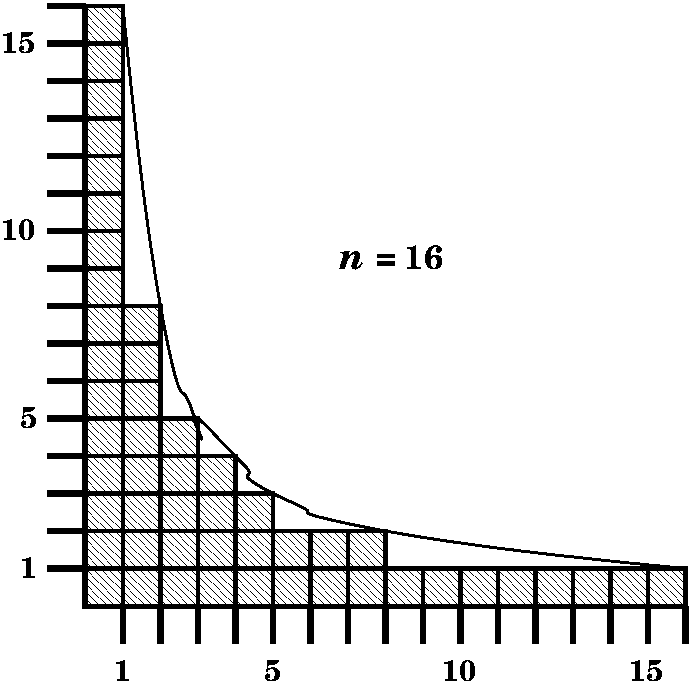
\includegraphics[scale=0.4]{pairing-hyp.pdf}
\caption{{\it The aggregate set of positions of tables having $16$ or
fewer position.}
\label{f.hyp}}
\end{figure}



\section{Arithmetic and Its Laws}\index{laws of arithmetic}
\label{sec:Arithmetic-Tools+Laws}

Numbers are {\it adjectives}\index{number!as adjective}---you have
five apples and three oranges---but in contrast to adjectives that are
purely descriptive---the red ball, the big dog---numbers can be {\em
  manipulated},\index{number!as {\em manipulable} adjective} using the
tools of {\it arithmetic}.

\subsection{The Tools of Arithmetic}
\label{sec:arithmetic-tools}

The basic tools of arithmetic reside in a small set of operations,
together with two special integers that play important roles with
respect to the operations.  Since these entities are so tightly
intertwined, we discuss them simultaneously.

\smallskip

\noindent {\small\sf Two special integers}
%
The integers zero ($0$)\index{number!zero ($0$)} and one
($1$),\index{number!one ($1$)} play special roles within all four of
the classes of numbers we have described.

\smallskip

\noindent {\small\sf  The operations of arithmetic}\index{arithmetic!basic operations}
%
Arithmetic on the four classes of numbers that we have described is
built upon a rather small repertoire of operations.  When we say that
an operation produces a number ``of the same sort'', we mean that it
produces
\begin{itemize}
\item
an integer result from integer arguments;
\item
a rational (number) result from rational (number) arguments;
\item
a real (number) result from real (number) arguments;
\item
a complex (number) result from complex (number) arguments;
\end{itemize}
The fundamental operations on numbers are, of course, familiar to the
reader.  Our goal in discussing them is to stress the laws that govern
the operations.  Along the way, we also introduce a few operations
that are less familiar but no less important.

\subsubsection{Unary (single-argument) operations}

\addcontentsline{toc}{paragraph}{A. Negating and reciprocating numbers}
\noindent {\small\sf A. Negating and reciprocating numbers.}
\index{arithmetic!basic operations!negation}
%
\noindent {\it i. The operation of {\em negation}}:
\index{arithmetic!basic operations!negating}
\begin{itemize}
\item
is a {\em total function} on the sets $\Z, \Q, \R, \C$.  It replaces
a number $a$ by its {\em negative},
\index{number!negative}
a number of the same sort, denoted $-a$.
\item
is a {\em partial function} on the nonnegative subsets
of $\Z, \Q, \R, \C$.  It replaces a number $a$ by its negative, $-a$,
whenever both $a$ and $-a$ belong to the nonnegative subset being
operated on.
\end{itemize}
Zero ($0$) is the unique {\it fixed point}\index{function!fixed
  point}\index{arithmetic!negation!fixed point} of the operation,
meaning that $0$ is the unique number $a$ such that $a = -a$.

\medskip

\noindent {\it ii. The operation of {\em reciprocation}}:
\index{arithmetic!basic operations!reciprocal}
\begin{itemize}
\item
\index{arithmetic!basic operations!reciprocating}
is a {\em total function} on the sets $\Q, \R, \C$, which replaces each
number $a$ by its {\em reciprocal}, 
\index{number!reciprocal}
a number of the same sort, denoted $1/a$ or $\displaystyle {1 \over
  a}$.  We shall employ whichever notation enhances legibility.

\item
is {\em undefined} on every integer $a$ except for $1$.
\end{itemize}

\medskip

\addcontentsline{toc}{paragraph}{B. Floors, ceilings, magnitudes}
\noindent {\small\sf B. Floors, ceilings, magnitudes.}
\index{arithmetic!basic operations!floor}
\index{arithmetic!basic operations!ceiling}
\index{arithmetic!basic operations!absolute value}
\index{arithmetic!basic operations!magnitude}

\noindent {\it i. The operations of {\em taking floors and ceilings}}
are total operations on the sets $\N, \Z, \Q, \R$.
\begin{itemize}
\item
The {\it floor} of a number $a$, also called {\it the integer part}
\index{arithmetic!basic operations!integer part of a number}
\index{arithmetic!basic operations!floor of a number}
of $a$, denoted $\lfloor a \rfloor$, is the largest integer that does
not exceed $a$; i.e.,:
\[
\lfloor a \rfloor \ \eqdef \ \max_{b \in {\mathbb{N}}} \Big[ b \ \leq a \Big]
\]
\item
The {\it ceiling} of a number $a$
\index{arithmetic!basic operations!ceiling of a number}
of $a$, denoted $\lceil a \rceil$, is the smallest integer that is 
not smaller than $a$:
\[
\lceil a \rceil \ \eqdef \ \min_{b \in {\mathbb{N}}} \Big[ b \ \geq a \Big]
\]
\end{itemize}
Thus, the operations of taking floors and ceilings are two ways to
{\em round} rationals and reals to their ``closest''
integers.\index{arithmetic!basic operations!rounding to ``closest'' integer}

\medskip

\noindent {\it ii. The operations of taking {\em absolute values/magnitudes}}:
\index{arithmetic!basic operations!absolute value, magnitude}
%
Let $a$ be a real number.  The {\it absolute value}, or, {\it
  magnitude}, of $a$, denoted $|a|$ equals either $a$ or $-a$,
whichever is positive.  For a complex number $a$, the definition of
$|a|$ is more complicated: it is a measure of $a$'s ``distance'' from
the ``origin'' complex number $0 + 0 \cdot i$.  In detail:
\[
|a| \ = \ \left\{
\begin{array}{cl}
a & \mbox{ if } \ [a \in \R] \ \ \mbox{ and } [a \geq 0] \\
-a & \mbox{ if } \ [a \in \R] \ \ \mbox{ and } [a < 0] \\
\sqrt{b^2 + c^2} &  \mbox{ if } \ [a \in \C]  \ \ \mbox{ and } [a = (b+ci)]
\end{array}
\right.
\]

\medskip

\addcontentsline{toc}{paragraph}{C. Factorials (of nonnegative integers)}
\noindent {\small\sf C. Factorials (of nonnegative integers).}
\index{arithmetic!basic operations!factorial (of a nonnegative integer)}
%
The {\it factorial} of a nonnegative integer $n \in \N$, which is
commonly denoted $n!$,
\index{arithmetic!basic operations!$n!$: factorial of $n \in \N$}
\index{arithmetic!basic operations!factorial of nonnegative integer}
is the function defined via the following recursion.
\begin{equation}
\label{eq:n-factorial-recursion}
\mbox{\sc fact}(n) \ = \ \left\{
\begin{array}{cl}
1 & \mbox{  if } \ n=0 \\
n \cdot \mbox{\sc fact}(n-1) & \mbox{  if } \ n>0
\end{array}
\right.
\end{equation}
By ``unwinding'' the recursion in (\ref{eq:n-factorial-recursion}),
one finds that, for all $n \in \N$,
\begin{equation}
\label{eq:n-factorial-direct}
n! \ = \ \mbox{\sc fact}(n) \ = \ 
n \cdot (n-1) \cdot (n-2) \cdot \cdots \cdot 2 \cdot 1
\end{equation} 
A $3$-step inductive argument validates this ``unwinding'':
\begin{enumerate}
\item
If $n =0$, then {\sc fact}$(n) = 1$, by definition
(\ref{eq:n-factorial-recursion}).
\item
Assume, for induction, that the expansion in
(\ref{eq:n-factorial-direct}) is valid for a given $k \in N$:
\[ \mbox{\sc fact}(k) \ = \ k \cdot (k-1) \cdot (k-2) \cdot \cdots
\cdot 2 \cdot 1 \] 
\item
Then:
\[
\begin{array}{lclll}
\mbox{\sc fact}(k+1) & = & (k+1) \cdot \mbox{\sc fact}(k)
  & & \mbox{by (\ref{eq:n-factorial-recursion})} \\
  & = &
(k+1) \cdot k \cdot (k-1) \cdot (k-2) \cdot \cdots \cdot 2 \cdot 1
  & & \mbox{by induction}
\end{array}
\]
\end{enumerate}


\subsubsection{Binary (two-argument) operations}
\label{sec:binary-operators}

%\addcontentsline{toc}{paragraph}{A. Addition and Subtraction}
\paragraph{\small\sf A. Addition and Subtraction.}
\index{arithmetic!basic operations!addition}
\index{arithmetic!basic operations!subtraction}
%
The operation of {\it addition}\index{arithmetic!addition} is a {\em
  total function} that replaces any two numbers $a$ and $b$ by a
number of the same sort.  The resulting number is the {\em sum of $a$
  and $b$}\index{arithmetic!addition!sum} and is denoted $a+b$.

\noindent
The operation of {\it subtraction}\index{arithmetic!subtraction} is a
{\em total function} on the sets $\Z, \Q, \R, \C$, which replaces any
two numbers $a$ and $b$ by a number of the same sort.  The resulting
number is the {\em difference of $a$ and $b$}
\index{arithmetic!subtraction!difference} and is denoted $a-b$.  On
the nonnegative subsets of the sets $\Z, \Q, \R, \C$---such as $\N$,
which is the largest nonnegative subset of $\Z$---subtraction is a
{\em partial function}, which is defined only when $a \geq b$.

Subtraction can also be defined as follows.  For any two numbers $a$
and $b$, {\em the difference of $a$ and $b$ is the sum of $a$ and the
  negation of $b$}; i.e.,
\[ a-b \ = \ a + (-b) \]

{\em The special role of $0$ under addition and subtraction.}
%
The number $0$ is the {\it identity} under addition and
  subtraction.\index{number!additive identity}\index{number!identity
  under addition}\index{identity!additive}
%
This means that, for all numbers $a$,
\[ a+0 \ = \ a-0 \ = \ a. \]

{\em The special role of $1$ under addition and subtraction.}
%
For any integer $a$, there is no integer between $a$ and $a+1$ or
between $a-1$ and $a$.  For this reason, on the sets $\Z$ and $\N$,
one often singles out the following special cases of addition and
subtraction, especially in reasoning about situations that are indexed
by integers.  Strangely, these operations have no universally accepted
notations.
\begin{itemize}
\item
The {\it successor} operation\index{arithmetic!integers!successor} is
a {\em total function} on both $\N$ and $\Z$, which replaces an
integer $a$ by the integer $a+1$.
\item
The {\it predecessor} operation\index{arithmetic!integers!predecessor}
is a {\em total function} on $\Z$, which replaces an integer $a$ by
the integer $a-1$.  It is a {\em partial function} on $\N$, which is
defined only when the argument $a$ is positive (so that $a-1 \in \N$).
\end{itemize}

The operations of addition and subtraction are said to be {\em
  inverse operations}\index{arithmetic!integers!additive inverse}
\index{arithmetic!integers!addition and subtraction are mutually
  inverse} of each other because each can be used to ``undo'' the
other:
\[
a \ = \ (a+b) -b \ = \ (a-b) +b
\]

\medskip

\addcontentsline{toc}{paragraph}{B. Multiplication and Division}
\noindent {\small\sf B. Multiplication and Division}.
\index{arithmetic!basic operations!multiplication}
\index{arithmetic!basic operations!division}
%
The operation of {\it multiplication}\index{arithmetic!multiplication}
is a {\em total function} that replaces any two numbers $a$ and $b$ by
a number of the same sort.  The resulting number is the {\em product
  of $a$ and $b$}\index{arithmetic!multiplication!product} and is
denoted either $a \cdot b$ \index{arithmetic!multiplication!$a \cdot  b$}
or $a \times b$.\index{arithmetic!multiplication!$a \times b$}
We shall usually favor the former notation, except when the latter
enhances legibility.

The operation of {\it division}\index{arithmetic!division} is a {\em
  partial function} on all of our sets of numbers.  Given two numbers
$a$ and $b$, the result of dividing $a$ by $b$---{\em when that result
  is defined}---is the {\it quotient of $a$ by $b$}
\index{arithmetic!division!When is $a/b$ defined?}
\index{arithmetic!division!quotient}
\index{arithmetic!division!quotient!$a/b$}
\index{arithmetic!division!quotient!$a \div b$}
\index{arithmetic!division!quotient!${a \over b}$}
and is denoted by one of the following three notations: $a/b$, $a \div
b$, $\displaystyle{a \over b}$.  The {\it quotient of $a$ by $b$} is
defined precisely when {\em both}

\noindent
\hspace*{.35in}(1) $b \neq 0$: one can never divide by $0$ \\
\hspace*{.35in}{\em and} \\
\hspace*{.35in}(2) there exists a number $c$ such that $a = b \cdot c$.

\noindent
Assuming that condition (1) holds, {\em condition (2) always holds
  when $a$ and $b$ belong to $\Q$ or $\R$ or $\C$}.

Division can also be defined as follows.  For any two numbers $a$
and $b$, {\em the quotient of $a$ and $b$ is the product of $a$ and the
reciprocal of $b$} (assuming that the latter exists); i.e.,
\[ a/b \ = \ a \cdot (1/b). \]
Computing reciprocals of nonzero numbers in $\Q$ and $\R$ is standard
high-school level fare; computing reciprocals of nonzero numbers in
$\C$ requires a bit of calculational algebra which we do not cover.
For completeness, we note that the reciprocal of the {\em nonzero}
complex number $a + bi \in \C$ is the complex number $c+di$ where
\[ c \ = \ \frac{a}{a^2 + b^2} \ \ \ \ \
\mbox{ and } \ \ \ \ \
d \ = \ \frac{-b}{a^2 + b^2}.
\]

{\em The special role of $1$ under multiplication and division.}
%
The number $1$ is the {\it identity} under the operations of
multiplication and division.\index{number!multiplicative
  identity}\index{number!identity under
  multiplication}\index{identity!multiplicative}
%
This means that, for all numbers $a$,
\[ a \cdot 1 \ = \ a \cdot (1/1) \ = \ a. \]

{\em The special role of $0$ under multiplication and division.}
%
The number $0$ is the {\it annihilator} under
multiplication.\index{multiplicative annihilator} This means that, for
all numbers $a$
\[ a \cdot 0 \ = \ 0. \]

The operations of multiplication and division are said to be {\em
  inverse operations}\index{arithmetic!integers!multiplicative
  inverse} \index{arithmetic!integers!multiplication and division are
  mutually inverse} because, when both operations can be applied, each
can be used to ``undo'' the other:
\[ a = (a \cdot b) \div b \ = \ (a \div b) \cdot b.  \]

\medskip

%\addcontentsline{toc}{paragraph}{C. Binomial coefficients and Pascal's triangle}
\paragraph{\small\sf C. Binomial coefficients and Pascal's triangle}
\index{arithmetic!basic operations!binomial coefficient}

We close our catalogue of arithmetic operations with a binary
operation on\footnote{In advanced contexts, one encounters binomial
  coefficients with non-integer arguments.}~$\N \times \N$.

Let $n$ and $k \leq n$ be nonnegative integers (i.e., elements of
$\N$).  The {\it binomial coefficient} denoted either as
$\displaystyle {n \choose k}$ or as $\Delta_{n,k}$, is the number
\index{binomial coefficients}
\begin{equation}
\label{eq:binom-coeff}
\Delta_{n,k} \ = \
{n \choose k} \ \eqdef \ \frac{n!}{k!(n-k)!} \ = \
\frac{n(n-1)(n-2) \cdots (n-k+1)}{k (k-1)(k-2) \cdots 1}
\end{equation}
Many of the secrets of these wonderful numbers---including the fact
that they are {\em integers}---can be deduced from the following
results.

\begin{prop}
\label{thm:manipulate-binom-coeff}
For all $n, k \in \N$ with $k \leq n$:

{\rm (a)} The symmetry rule:
\index{binomial coefficients!symmetry rule}
\begin{equation}
\label{eq:symmetry-binom-coeff}
{n \choose k} \ = \ {n \choose {n-k}}
\end{equation}

{\rm (b)} The addition rule:
\index{binomial coefficients!addition rule}
\begin{equation}
\label{eq:add-binom-coeff}
{n \choose k} \ + \ {n \choose {k+1}} \ = \ {{n+1} \choose {k+1}}
\end{equation}
\end{prop}

\begin{proof}
($a$)
We verify equation (\ref{eq:symmetry-binom-coeff}) by
(\ref{eq:binom-coeff}) plus the commutativity of multiplication (see
Section~\ref{sec:Arithmetic-Laws}),
\begin{eqnarray*}
{n \choose k} & = & \frac{n!}{k!(n-k)!} \\
              & = & \frac{n!}{(n-k)!k!} \\
              & = & {n \choose {n-k}}
\end{eqnarray*}

\noindent ($b$)
We verify equation (\ref{eq:add-binom-coeff}) by explicitly adding the
fractions exposed by (\ref{eq:binom-coeff}):
\begin{eqnarray*}
{n \choose k} \ + \ {n \choose {k+1}}
  & = &
\frac{n!}{k!(n-k)!} \ + \ \frac{n!}{(k+1)!(n-k-1)!} \\
  & = &
n! \cdot \frac{(k+1) + (n-k)} {(k+1)!(n-k)!} \\
  & = & 
\frac{(n+1)!}{(k+1)!(n-k)!} \\
  & = &
{{n+1} \choose {k+1}} \hspace*{2in} \qed
\end{eqnarray*}

Extrapolating from Proposition~\ref{thm:manipulate-binom-coeff}, we now
present {\it Pascal's triangle}, named in honor of
\index{Pascal's triangle}
\index{Pascal, Blaise}
the French polymath Blaise Pascal.  Fig.~\ref{fig:pascal-triangle}
provides a ``prefix'' of this famed array of integers, for $n,k \leq
5$.
\begin{figure}[htb]
\[
\begin{array}{c||r|r|r|r|r|r|r}
{\displaystyle {n \choose k}} & k=0 & k=1 & k=2 & k=3 & k=4 & k=5 &\ldots \\
\hline
\hline
n=1 & 1 & 1 &    &    &    &   & \ldots \\
\hline
n=2 & 1 & 2 & 1  &    &    &   & \ldots \\
\hline
n=3 & 1 & 3 & 3  & 1  &    &   & \ldots \\
\hline
n=4 & 1 & 4 & 6  & 4  & 1  &   & \ldots \\
\hline
n=5 & 1 & 5 & 10 & 10 & 5  & 1 & \ldots \\
\hline
\vdots &\vdots &\vdots &\vdots &\vdots &\vdots &\vdots &\ddots
\end{array}
\]
\caption{A ``prefix'' of Pascal's Triangle, for $n,k \leq 5$.}
\label{fig:pascal-triangle}
\end{figure}
The formation rule of the array is:
\begin{description}
\item[\sf Formation rule for Pascal's triangle:]
% 
{\it The entry at (row $n+1$, column $k+1$) is the sum of the entries
  at (row $n$, column $k$) and (row $n$, column $k+1$).}
\end{description}
\qed
\end{proof}


If you compare the formation rule for Pascal's triangle with equation
(\ref{eq:add-binom-coeff}), then you may anticipate the following
result.

\addcontentsline{toc}{paragraph}{-- A fun result: Pascal's triangle
  and the binomial coefficients}

\begin{prop}
\label{thm:pascal-binom}
The entries of Pascal's triangle are the binomial coefficients.
Specifically, for all $n,k$, the entry at (row $n$, column $k$) of the
Triangle is $\displaystyle {n \choose k}$.
\end{prop}

\begin{proof}
We note by observation and direct calcullation (see
Fig.~\ref{fig:pascal-triangle}) that the proposition is true for $n =
1$ and $k \in \{0, 1\}$.  A simple double induction

\noindent
****************** \\
induction on $n$, then for each value of $n$ on $k \leq n$ \\
SHOULD WE SPELL THIS OUT IN DETAIL?  GIVE AS AN EXERCISE? \\
******************

\noindent
verifies that every binomial coefficient appears in the Triangle and
every Triangle entry is a binomial coefficient.  \qed
\end{proof}

\medskip

\addcontentsline{toc}{paragraph}{-- A fun result: Binomial
  coefficients are integers}

\begin{prop}
\label{thm:binomcoeff-integer}
Every binomial coefficient is an integer.
\end{prop}

\begin{proof}
Since every entry in Pascal's triangle is obtained from integers via
repeated additions, this result follows from
Proposition~\ref{thm:pascal-binom}.  \qed
\end{proof}

\bigskip

Binomial coefficients are indispensable when studying myriad topics
related to {\em counting}, such as:
\begin{itemize}
\item
what are the relative likelihoods of various $5$-card deals from a
fair $52$-card deck?
\item
What is the likelihood of observing $15$ {\sc head}s and $25$ {\sc
  tail}s in $40$ flips of a fair coin?
\item
What are the comparative operation-count costs of Merge-Sort and
Quick-Sort when sorting $n$ keys; cf.~\cite{CLRS}?

\end{itemize}
We shall, therefore, see a lot more about binomial coefficients in
Section~\ref{sec:powers+polynolmials} and Chapter~\ref{ch:prob-stat}.
With each subsequent encounter, our respect for these numbers will
grow.


\subsection{The Laws of Arithmetic, and applications}
\index{arithmetic!basic laws}
\label{sec:Arithmetic-Laws}

The student should understand the following laws of arithmetic on the
reals, rationals, and reals---and be able to employ them cogently in
rigorous argumentation.

\medskip

\addcontentsline{toc}{paragraph}{A. The commutative law}
\noindent {\small\sf A. The commutative law.}
\index{commutative law!arithmetic}
\index{commutative law!addition}
\index{commutative law!multiplication}
\index{arithmetic!commutative law}
%
For all numbers $x$ and $y$:
\[
\begin{array}{llc}
\mbox{\it for addition:}
  & & x+y \ = \ y+x \\
\mbox{\it for multiplication:}
  & & x \cdot y \ = \ y \cdot x
\end{array}
\]

\medskip

\addcontentsline{toc}{paragraph}{B. The associative law}
\noindent {\small\sf B. The associative law}
\index{associative law for arithmetic}
\index{arithmetic!associative law}
%
For all numbers $x$, $y$, and $z$,
\[ (x+y)+z \ = \ x+(y+z) \ \ \ \mbox{\bf and } \ \ 
x\cdot (y\cdot z) 
(x \cdot y) \cdot z \ = \ x\cdot (y\cdot z). \] 
This allows one, for instance, to write strings of additions or of
multiplications without using parentheses for grouping.

\medskip

\addcontentsline{toc}{paragraph}{C. The distributive law}
\noindent  {\small\sf C. The distributive law.}
\index{distributive law for arithmetic}
\index{arithmetic!distributive law}
%
For all numbers $x$, $y$, and $z$,
\begin{equation}
\label{eq:distr-law}
x \cdot (y + z) \ = \ (x \cdot y) + (x \cdot z).
\end{equation}
One commonly articulates this law as, ``{\em Multiplication
  distributes over addition.}''


One of the most common uses of the distributive law reads equation
(\ref{eq:distr-law}) ``backwards,'' thereby deriving a formula for
{\em factoring} \index{arithmetic!factoring} complex expressions that
use both addition and multiplication.

Easily, addition does {\em not} distribute over multiplication; i.e.,
in general, $x + y \cdot z \ \neq \ (x+y) \cdot (x+z)$.  Hence, when
we see ``$x + y \cdot z$'', we know that the multiplication is
performed before the addition.  In other words, {\em Multiplication
  takes priority over addition.}  \index{arithmetic!priority of
  multiplication over addition} This priority permits us to write the
righthand side of (\ref{eq:distr-law}) without parentheses, as in
\[ x \cdot (y + z) \ = \ x \cdot y + x \cdot z. \]

Via multiple invocations of the preceding laws, we can derive a recipe
for multiplying complicated expressions.  We illustrate this via the
``simplest'' complicated expression, $(a+b) \cdot (c+d)$.

\begin{prop}
\label{prop:(a+b)(c+d)}
For all numbers $a, b, c, d$:
\begin{equation}
\label{eq:(a+b)(c+d)}
(a+b) \cdot (c+d) \ = \ a \cdot c + a \cdot d + b \cdot c + b \cdot d
\end{equation}
\end{prop}

\begin{proof}
Note first that because multiplication takes priority over addition,
the absence of parentheses in expressions such as
(\ref{prop:(a+b)(c+d)}) does not jeopardize unambiguity.  Our proof of
the proposition invokes the laws we have just enunciated multiple
times.
\[
\begin{array}{lclll}
(a+b) \cdot (c+d) & = & (a+b) \cdot c \ + \ (a+b) \cdot d
& & \mbox{distributive law} \\ 
  & = & c \cdot (a+b) \ + \ d \cdot (a+b)
& & \mbox{commutativity of multiplication} \ (2 \times) \\
  & = & c \cdot a + c \cdot b + d \cdot a + d \cdot b 
& & \mbox{distributive law} \ (2 \times) \\
  & = & a \cdot c + b \cdot c + a \cdot d + b \cdot d
& & \mbox{commutativity of multiplication} \ (4 \times) \\
  & = &  a \cdot c + a \cdot d + b \cdot c + b \cdot d
& & \mbox{commutativity of addition}
\end{array}
\]
\qed
\end{proof}


We close our short survey of the laws of arithmetic with the following
important two-part law.
\begin{itemize}
\item
{\it The law of inverses}.\index{inverse laws for
  arithmetic}\index{laws of arithmetic!inverse laws}
%
  \begin{itemize}
  \item
Every number $x$ has an {\em additive inverse},\index{additive inverse}
i.e., a number $y$ such that $x+y =0$.  This inverse is $x$'s {\it
  negative} $-x$.\index{additive inverse!negative as additive inverse}
  \item
Every {\em nonzero} number $x \neq 0$ has a {\em multiplicative
  inverse},\index{multiplicative inverse} i.e., a number $y$ such that
$x \cdot y = 1$.  This inverse is $x$'s {\it reciprocal},
$1/x$.\index{multiplicative inverse!reciprocal as multiplicative inverse}
  \end{itemize}
\end{itemize}

We close this section with another of our ``fun'' propositions.

\addcontentsline{toc}{paragraph}{-- A fun result: A ``trick'' for
  squaring some integers}

\begin{prop}
\label{thm:75x65=4925}
Let $n$ be any number that has a $2$-digit decimal of the form $\delta
5$, where $\delta \in \{ 0,1,2,3,4,5,6,7,8,9 \}$,
so that
\[ n \ = \ 10 \cdot \delta + 5
\]
Then 
\[ n^2 \ = \ 100 \cdot \delta \cdot (\delta+1) + 25. \]
In other words, one obtains a base-$10$ numeral for $n^2$ by
multiplying $\delta$ by $\delta +1$ and appending $25$ to the product.
\end{prop}

\noindent
Examples of Proposition ~\ref{thm:75x65=4925} include
$25^2 = 625$ (because $2 \cdot 3 = 6$) and $75^2 = 5625$ (because $7
\cdot 8 = 56$).

\begin{proof} (for general $\delta$).
%
We invoke Proposition~\ref{prop:(a+b)(c+d)} and the distributive law.
\[
\begin{array}{lclll}
n^2 & = & (10 \cdot \delta + 5)^2 & & \mbox{Given} \\
    & = & 100 \cdot \delta^2 \ + \ 100 \cdot delta \ + \ 25
              & & \mbox{the proposition} \\
    & = & 100 \cdot (\delta^2 \ + \ \delta) \ + \ 25
              & & \mbox{factoring: distributive law} \\
    & = & 100 \cdot \delta \cdot (\delta + 1) \ + \ 25
              & & \mbox{factoring: distributive law} \\
\end{array}
\]
\qed
\end{proof}


\subsection{Rational Arithmetic: A Worthwhile Exercise}
\label{sec:Rational-arithmetic}
\index{number!rational!arithmetic}

In Section~\ref{sec:rationals} we defined the rational numbers and
reviewed why they were needed to compensate for the general lack of
multiplicative inverses in the integers.  But we did not review how to
perform arithmetic on the elements of the set $\Q$.  We correct this
shortcoming now.  Of course, the reader will have encountered rational
arithmetic long ago---but we are now reviewing the topic in order to
provide the reader with a set of worthwhile exercise to reinforce the
mathematical thinking whose presentation is our main goal.

\medskip

The rational numbers build their rules for arithmetic upon the
corresponding rules for integers.  For all $p/q$ and $r/s$ in $\Q$:
\[
\begin{array}{|llcl|}
\hline
\mbox{\small\sf Addition:} & 
{\displaystyle
{p \over q} + {r \over s} }
  & = &
{\displaystyle
 \frac{p \cdot s + r \cdot q}{q \cdot s} }  \\
 & & & \\
\mbox{\small\sf Subtraction:} &
{\displaystyle
{p \over q} + {r \over s} }
  & = & 
{\displaystyle
{p \over q} + {(-r) \over s} } \\
 & & & \\
\mbox{\small\sf Multiplication:} &
{\displaystyle
{p \over q} \cdot {r \over s} }
  & = & 
{\displaystyle
\frac{p \cdot r}{r \cdot s} } \\
  & & & \\
\mbox{\small\sf Division:} &
{\displaystyle
{p \over q} \div {r \over s} }
  & = &
{\displaystyle
{p \over q} \cdot {s \over r} } \\
\hline
\end{array}
\]

It is worth verifying that rational arithmetic as thus defined behaves
in the required manner; in particular that rational arithmetic:
\begin{itemize}
\item
works correctly when the argument rational numbers are, in fact,
integers, i.e., when $q = s = 1$ in the preceding table.
\item
treats the number $0$ appropriately, i.e., as an additive identity and
a multiplicative annihilator; cf., Sections~\ref{sec:arithmetic-tools}
and~\ref{sec:Arithmetic-Laws}.
\item
obeys the required laws; cf., Section~\ref{sec:Arithmetic-Laws}.

Verifying the distributivity of rational multiplication over rational
addition will be a particularly valuable exercise because of the
required amount of manipulation.
\end{itemize}

\section{Basic Algebraic Concepts and Their Manipulations}

\subsection{Powers and polynomials}
\label{sec:powers+polynolmials}

\subsubsection{Raising a number to a power.}
\label{sec:x-toa-power}
A conceptually powerful notational construct is the operation of {\it
  raising a number to a power:}\index{raising a number to a power}
%
For real numbers $a$ and $b$, the {\it $b$th power} of $a$, denoted
$a^b$ is defined by the system of equations
\begin{equation}
\label{eq:power-def}
\begin{array}{llll}
\mbox{for all numbers $a>0$} & & & a^0 = 1 \\
 & & & \\
\mbox{for all numbers $a, b, c$} & & & a^b \cdot a^c = a^{b+c}.
\end{array}
\end{equation}
This deceptively simple definition has myriad consequences which we
often take for granted.
\begin{itemize}
\item
For all numbers $a>0$, the number $a^0 = 1$.

This follows (via cancellation) from (\ref{eq:power-def}) via the fact
that
\[ a^b \cdot a^0 \ = \ a^{b+0} \ = \ a^b \ = \ a^b \cdot 1.  \]

\item
For all numbers $a >0$, the number $a^{1/2}$\index{$a^{1/2}$: the
  square root of number $a$}
is the {\it square root} of $a$,\index{square root}
i.e., $a^{1/2}$ is the (unique, via cancellation) number $b$ such that
$b^2 = a$.  Another common notation for The number $a^{1/2}$ is
$\sqrt{a}$.\index{$\sqrt{a}$: the square root of number $a$}

This follows from (\ref{eq:power-def}) via the fact that
\[ a \ = \ a^1 \ = \ a^{(1/2) + (1/2)} \ = \ a^{1/2} \cdot a^{1/2} \ = \
\left(a^{1/2}\right)^2. \]

\item
For all numbers $a>0$ and $b$, the number $a^{-b}$ is the {\it
  multiplicative inverse}\index{multiplicative inverse}
of $a^b$, meaning that $a^b \cdot a^{-b} = 1$

This follows from (\ref{eq:power-def}) via the fact that
\[ a^b \cdot a^{-b} \ = \ a^{(b + (-b))} \ = \ a^0 \ = \  1 \]
\end{itemize}
When the power $b$ is a positive integer, then definition
(\ref{eq:power-def}) can be cast in the following attractive inductive
form:
\begin{equation}
\label{eq:power-def-integer}
\begin{array}{llll}
\mbox{for all numbers $a>0$} & & & a^0 = 1 \\
 & & & \\
\mbox{for all numbers $a$ and integers $b$} & & & a^{b+1} = a \cdot
a^b.
\end{array}
\end{equation}
Summing up, we now know about powers that are integral or fractional,
positive, zero, or negative

\subsubsection{Polynomials and their roots.}
\label{sec:poly-roots}
We want students to master the notions of polynomials and their
associated notions, such as degrees and coefficients, and computations
therewith, including polynomial summation and multiplication.  While
polynomial multiplication is often considered ``non-elementary'', it
must be mastered in order to fully understand positional number
systems; it is also essential, e.g., when discussing a range of topics
relating to, say, fault tolerance and encryption).

\index{The Fundamental Theorem of Algebra}
\begin{theorem}[The Fundamental Theorem of Algebra]
Every degree-$n$ univariate polynolmial with complex coefficients has
$n$ complex roots 
\end{theorem}

\index{The Binomial Theorem}
\subsubsection{The Binomial Theorem.}
\label{sec:Binomial-thm}

Perhaps the simplest bivariate polynomials are the ones in the
following family.
\begin{equation}
\label{eq:binomial-polys}
\mbox{For } \ n \in \N^+, \hspace*{.5in}
P_n(x,y) \ \eqdef \ (x+y)^n.
\end{equation}
There are lessons to be learned from the structure of these
polynomials, so let us begin to expand them using the arithmetic
techniques we have learned earlier.
\begin{eqnarray*}
P_1(x,y) \ = \
(x+y)^1 & = & x+y  \\
P_2(x,y) \ = \
(x+y)^2 & = & (x+y) \cdot (x+y) \\
        & = & x^2 + 2xy + y^2 \\
P_3(x,y) \ = \
(x+y)^3 & = & (x+y) \cdot (x^2 + 2xy + y^2) \\
   & = & (x^3 + 2x^2y +  xy^2) + (x^2y + 2xy^2 + y^3) \\
   & = & x^3 + 3x^2y + 3xy^2 + y^3  
\end{eqnarray*}

Let us stop to review what we are seeing.  We have remarked before
that doing mathematics can sometimes involve a wonderfully exciting
(quite sophisticated) pattern-matching game.  So, let us pattern-match!
\begin{enumerate}
\item
The coefficients of the expanded $P_1(x,y)$ are $\langle 1,1 \rangle$.
\item
The coefficients of the expanded $P_2(x,y)$ are $\langle 1,2,1 \rangle$.
\item
The coefficients of the expanded $P_3(x,y)$ are $\langle 1,3,3,1 \rangle$.
\end{enumerate}
There is a pattern emerging here.  Can you spot it?  Where have we
seen a pattern of tuples that begins in the same manner?  As a rather
broad hint, look at Fig.~\ref{fig:pascal-triangle}!  Could the
coefficients of each $P_n$ possibly be the successive binomial
coefficients
\[ {n \choose 0}, \ {n \choose 1}, \ \ldots, \ {n \choose {n-1}}, \ {n
  \choose n}
\]
Let us use induction to explore this possibility by expanding a
generic $P_n$ with symbolic ``dummy'' coefficients and see what this
says about $P_{n+1}$.  To this end, let $a_{n,n-r}$ denote the
coefficient of $x^{n-r} y^r$ in the expansion of $P_n(x,y)$.  Using
our ``dummy'' coefficients, we have
\[ 
\begin{array}{l}
P_n(x,y) \ = \
 x^n \ + \ \cdots \ + \ a_{n,n-r} x^{n-r} y^r
    \ + \ a_{n,n-r-1} x^{n-r-1} y^{r+1} \\
\hspace*{1in} + \ a_{n,n-r-2} x^{n-r-2} y^{r+2}
 \ + \ \cdots \ + \ y^n
\end{array}
\]
Continuing with this symbolic evaluation, we have:
\begin{equation}
\label{eq:xPk}
\begin{array}{l}
x \cdot P_n(x,y) \ = \
 x^{n+1} \ + \ \cdots \ + \ a_{n,n-r} x^{n-r+1} y^r
    \ + \ a_{n,n-r-1} x^{n-r} y^{r+1} \\
\hspace*{1in} + \ a_{n,n-r-2} x^{n-r-1} y^{r+2}
 \ + \ \cdots \ + \ xy^n
\end{array}
\end{equation}
and
\begin{equation}
\label{eq:yPk}
\begin{array}{l}
y \cdot P_n(x,y) \ = \
 x^n y \ + \ \cdots \ + \ a_{n,n-r} x^{n-r} y^{r+1}
    \ + \ a_{n,n-r-1} x^{n-r-1} y^{r+2} \\
\hspace*{1in} + \ a_{n,n-r-2} x^{n-r-2} y^{r+3}
 \ + \ \cdots \ + \ y^{n+1}
\end{array}
\end{equation}
Because
\[ P_{n+1}(x+y) \ = \ (x+y) \cdot P_n(x,y)
                \ = \ x \cdot P_n(x,y) \ + \ y \cdot P_n(x,y),
\]
the ``dummy'' coefficient $a_{n-r+1,r}$ of $x^{n-r+1} y^r$ in
$P_{n+1}(x+y)$ is the sum of the following coefficients in $P_n(x,y)$:
\begin{center}
$\bullet$
the coefficient $a_{n,n-r}$ of $x^{n-r}y^r$ \ \ \ \ \
and \ \ \ \ \
$\bullet$
the coefficient $a_{n,n-r+1}$ of $x^{n-r+1}y^{r-1}$
\end{center}
By induction, then, for all $n,r \in \N$ with $r \leq n$,
\[ a_{n,r} + a_{n,r+1} \ = \ a_{n+1,r+1} \]
Combining this equation with the observed initial conditions
\[ a_{1,0} \ = \ a_{1,1} \ = \ 1 \]
we see that each coefficient $a_{n,r}$ is actually the binomial
coefficient $\displaystyle {n \choose r}$.  This observation is
attributed to the renowned English mathematician/physicist Isaac
Newton and is enshrined in Newton's famous {\it Binomial Theorem}.

\ignore{**********
so that, finally,
\begin{eqnarray*}
             & = &
 x^{k+1} \ + \ (k+1) x^k y \ + \ \cdots \ + \
   (a_{k,k-r-1} + a_{k,k-r}) x^{k-r} y^{r+1} \\
             &   & \ \ \ + \
   (a_{k,k-r-2} + a_{k,k-r-1}) x^{k-r-1} y^{r+2}
 \ + \ \cdots \ + \ (k+1) xy^k \ + \ y^{k+1} \\
      & = &
 x^{k+1} \ + \ (k+1) x^k y \ + \ \cdots \ + \
 a_{k+1,k-r} x^{k-r} y^{r+1} \\
            &    & \ \ \ + \  a_{k+1,k-r-1} x^{k-r-1} y^{r+2}
 \ + \ \cdots \ + \ (k+1) xy^k \ + \ y^{k+1}
\end{eqnarray*}
*******}

\begin{theorem}[The Binomial Theorem]
\label{thm:Binomial-theorem}
For all $n \in \N$,
\[
(x+y)^n \ = \
\sum_{i=0}^n \ \ {n \choose i} x^{n-i} y^i.
\]
\end{theorem}
\index{The Binomial Theorem!binomial coefficients}
\index{binomial coefficients!The Binomial Theorem}



\subsection{Exponentials and Logarithms}
\label{sec:exponential+logarithm}

This section introduces the fundamentals of two extremely important
classes of functions which are functional inverses of each other, in
the following sense.  Functions $f$ and $g$ are {\it functional
  inverses}\index{functional inverse} of each other if for all
arguments $x$
\begin{equation}
\label{eq:functional-inverse}
f(g(x)) \ = \ x.
\end{equation}

\subsubsection{Basic definitions}

\paragraph{\small\sf A. Exponential functions}.\index{Exponential functions}
%
A function $f$ is {\it exponential} if there is a positive number $b$
such that, for all $x$,
\begin{equation}
\label{eq:exponential-defn}
f(x) \ = \ b^x.
\end{equation}
The number $b$ is the {\it base}\index{base of exponential}
%
of $f(x)$.  The basic arithmetic properties of exponential functions
are derivable from (\ref{eq:power-def}), so we leave these details to
the reader and turn immediately to the functional inverses of
exponential functions..

\paragraph{\small\sf B. Logarithmic functions}.\index{Logarithmic
  functions}
%
Given an integer $b >1$ (mnemonic for ``base''), the {\em base-$b$
  logarithm}\index{base-$b$ logarithm}
%
of a real number $a > 0$ is denoted $\log_b a$ and defined by the
equation\index{$\log_b a$: the base-$b$ logarithm of number $a$}
\begin{equation}
\label{eq:logarithm-defn}
a \ = \ b^{\log_b a}.
\end{equation}
Logarithms are partial functions: $\log_b a$ is not defined for
non-positive arguments.

The base $b = 2$ is so prominent in the contexts of computation theory
and information theory that we commonly invoke one of two special
notations for $\log_2 a$: (1) we often elide the base-$2$ subscript
and write $\log a$;\index{$\log(a)$: base-$2$ logarithm of number $a$}
(2) we employ the specialized notation $\ln a$\index{$\ln(a)$:
  base-$2$ logarithm of number $a$}.  Notationally:
\[ \log_2 a \ \eqdef \ \log a \ \eqdef \ \ln a \]

We leave to the reader the easy verification, from
(\ref{eq:logarithm-defn}), that the {\it base-$b$ logarithmic
  function}, defined by
\begin{equation}
\label{eq:log-function-defn}
f(x) \ = \ \log_b x
\end{equation}
is the functional inverse of the base-$b$ exponential function.

\subsubsection{Fun facts about exponentials and logarithms}

Definition (\ref{eq:logarithm-defn}) exposes and---even more
importantly---explains myriad facts about logarithms that we often
take for granted.

\begin{prop}
For any base $b >1$, for all numbers $x >0$, $y>0$,
\[ \log_b (x \cdot y) \ = \ \log_b x \ + \ \log_b y \]
\end{prop}

\begin{proof}
Definition (\ref{eq:logarithm-defn}) tells us that $x = b^{\log_b x}$
and $y = b^{\log_b y}$.  Therefore,
\[ x \cdot y \ = \ b^{\log_b x} \cdot b^{\log_b y} \ = \
b^{\log_b x \ + \ \log_b y}, \]
by the laws of powers.  Taking base-$b$ logarithms of the first and
last terms in the chain yields the claimed equation.
\qed
\end{proof}



Many students believe that the following result is a {\em convention}
rather than a consequence of the basic definitions.  {\em The logarithm
  of $1$ to any base is $0$.}

\begin{prop}
For any base $b >1$,
\[ \log_b 1 \ = \ 0 \]
\end{prop}

\begin{proof}
We note the following chain of equalities.
\[  b^{\log_b x} \ = \ b^{\log_b (x \cdot 1)} 
\ = \ b^{(\log_b x) + (\log_b 1)} 
\ = \ b^{\log_b x} \cdot b^{\log_b 1}
\]
Hence, $b^{\log_b 1} \ = \ 1$.  If $\log_b 1$ did not equal $0$, then
$b^{\log_b 1}$ would exceed $1$.  \qed
\end{proof}

\begin{prop}
For all bases $b > 1$ and all numbers $x, y$,
\[ x^{\log_b y} \ = \ y^{\log_b x} \]
\end{prop}

\begin{proof}
We invoke (\ref{eq:logarithm-defn}) twice to remark that
\[ \left[x^{\log_b y} \ = \ b^{(\log_b x) \cdot (\log_b y)}\right]
\ \ \mbox{ and } \ \ 
\left[y^{\log_b x}\ = \ b^{(\log_b y) \cdot (\log_b x)}\right] \]
The commutativity of addition completes the verification.  \qed
\end{proof}

\begin{prop}
For any base $b >1$,
\[ \log_b (1/x) \ = \ - \log_b x \]
\end{prop}

\begin{proof}
This follows from the fact that $\log_b 1 =0$, coupled with the
product law for logarithms.
\[ \log_b x + \log_b (1/x) \ = \ \log_b (x \cdot (1/x))
\  = \ \log_b 1 \ = \ 0 
\]
\qed
\end{proof}

\begin{prop}
For any bases $a, b >1$,
\begin{equation}
\label{eq:log-exp-0}
\log_b x \ = \ \left(\log_b a \right) \cdot \left( \log_a x \right).
\end{equation}
\end{prop}

\begin{proof}
We begin by noting that, by definition,
Note that
\begin{equation}
\label{eq:log-exp-1}
 x \ = \ b^{\log_b x} \ = \ a^{\log_a x} .
\end{equation}
Let us take the base-$b$ logarithm of the second and third expressions
in (\ref{eq:log-exp-1}) and then invoke the product law for logarithms.
From the second expression in (\ref{eq:log-exp-1}), we find that
\begin{equation}
\label{eq:log-exp-2}
 \log_b \left(b^{\log_b x} \right) \ = \ \log_b x .
\end{equation}
From the third expression in (\ref{eq:log-exp-1}), we find that
\begin{equation}
\label{eq:log-exp-3}
 \log_b \left( a^{\log_a x} \right) \ = \
\left(\log_b a \right) \cdot \left( \log_a x \right).
\end{equation}
We know from (\ref{eq:log-exp-1}) that the righthand expressions in
(\ref{eq:log-exp-2}) and (\ref{eq:log-exp-3}) are equal, whence
(\ref{eq:log-exp-0}).   \qed
\end{proof}

If we set $x = b$ in (\ref{eq:log-exp-0}), then we find the following
marvelous equation.

\begin{prop}
For any integers $a, b >1$,
\begin{equation}
\left(\log_b a \right) \cdot \left( \log_a b \right) \ = \ 1 \ \ \ \ \
\mbox{ or, equivalently, } \ \ \ \ \
\log_b a \ = \ \frac{1}{\log_a b} .
\end{equation}
\end{prop}


\subsubsection{Exponentials and logarithms within information theory}
\label{sec:count-strings}

The student should recognize and be able to reason about the following
facts.  If one has an alphabet of $a$ letters/symbols and must provide
distinct string-label ``names'' for $n$ items, then at least one
string-name must have length no shorter than $\lceil \log_a n \rceil$.

\begin{prop}
\label{thm:bound-stringnames-lgth-k}
Say that one must assign distinct labels to $n$ items, via strings
over an alphabet of $a$ letters.  Then at least one string-label must
have length no shorter than $\lceil \log_a n \rceil$.
\end{prop}

\begin{proof}
Let $Sigma$ be an alphabet of $a$ letters/symbols.  For each integer
$k \geq 0$ (i.e., for each $k \in \N$), let $\Sigma^{(k)}$ denote the
set of all length-$k$ strings over $\Sigma$.  The bound of
Proposition~\ref{thm:bound-stringnames-lgth-k} follows by counting the
number of strings of various lengths over $\Sigma$, because each such
string can label at most one item.  Let us, therefore, inductively
evaluate the cardinality $|\Sigma^{(k)}|$ of each set $\Sigma^{(k)}$.
\begin{itemize}
\item
$|\Sigma^{(0)}| =1$

This is because the null-string $\varepsilon$ \index{$\varepsilon$:
  the null string, of length $0$}
\index{null string $\varepsilon$}
is the unique string in $\Sigma^{(0)}$, i.e., $\Sigma^{(0)} = \{
\varepsilon \}$.

\item
$|\Sigma^{(k+1)}| = |Sigma| \cdot |\Sigma^{(k)}|$.

This reckoning follows from the following recipe for creating all
strings over $\Sigma$ of length $k+1$ from all strings of length $k$.
\[
\Sigma^{(k+1)} \ = \ \{ \sigma x \ | \ \sigma \in \Sigma, x \in
\Sigma^{(k)} \}
\]
This recipe is correct because
  \begin{itemize}
  \item
Each string in $\Sigma^{(k+1)}$, as constructed, has length $k+1$.

This is because the recipe adds a single symbol to a length-$k$
string.
  \item
For each string $x \in \Sigma^{(k)}$, there are $|\Sigma|$ distinct
strings in $\Sigma^{(k+1)}$, as constructed.

This is because each string in $\Sigma^{(k+1)}$ begins with a distinct
symbol from $\Sigma$.

  \item
$\Sigma^{(k+1)}$, as constructed, contains all strings of length $k+1$
over $\Sigma$.

This is because for each $\sigma \in \Sigma$ and each $x \in
\Sigma^{(k)}$, the string $\sigma x$ is in $\Sigma^{(k+1)}$, as
constructed.
  \end{itemize}
\end{itemize}
We thus have the following recurrence.
\begin{eqnarray*}
|\Sigma^{(0)}| & = & 1 \\
|\Sigma^{(k+1)}| & = & |\Sigma| \cdot |\Sigma^{(k)}| \ \ \ \ 
\mbox{ for } \ k \geq 0
\end{eqnarray*}
Using the Master Theorem, we thus find explicitly that

\noindent
For each $\ell \in \N$,
\[ |\Sigma^{(\ell)}| \ = \ \frac{|\Sigma|^{\ell+1} \ - \ |\Sigma|}
{|\Sigma| -1} \ \leq \ c \cdot |\Sigma|^{\ell}
\]
for some constant $c$.  In order for this quantity to reach $n \in
\N$, we must have
\[ \ell \ > \ d \cdot \log_{|\Sigma|} n   \]
for some small constant $d$.  \qed
\end{proof}

**HERE

Focus on 
Say, inductively, that there are $\ell_k$


\begin{prop}
\label{thm:Num-strings-lgth-k}
The number of distinct strings of length $k$ over an alphabet of $a$
letters is $a^k$.
\end{prop}


\ignore{*********************

\subsection{Arithmetic and geometric sequences and series}
\label{sec:sums-series}

The ability to sum -- and perhaps approximate -- simple series,
including, {\em at least}, finite arithmetic series and both finite
and infinite geometric series.

\subsubsection{Arithmetic sequences and series.}
\label{sec:arithmetic-series}
%
We define arithmetic sequences and learn how to calculate their sums.

\begin{equation}
\label{eq:arith-seq}
\begin{array}{l}
\mbox{An $n$-term arithmetic sequence:} \\
\hspace*{.25in}a, \ a+b, \ a+2b, \ a+3b, \ \ldots, a+(n-1)b \\
\\
\mbox{The corresponding arithmetic series:} \\
\hspace*{.25in}a + (a+b) + (a+2b) + (a+3b) + \cdots + (a+(n-1)b) \\
\hspace*{.5in} = \
an + b \cdot (1 + 2 + \cdots + n-1)
\end{array}
\end{equation}
We can, thus, sum the arithmetic series in (\ref{eq:arith-seq}) by
determining the sum of the first $m$ positive integers; $m = n-1$ in
(\ref{eq:arith-seq}).  We use this result as an opportubnity to
introduce important notation.

\addcontentsline{toc}{paragraph}{-- A fun result: Summing the first
  $n$ integers}

\begin{prop}
\label{thm:sum-first-integers-Gauss}
For all $n \in \N$,
\begin{eqnarray}
\nonumber
S_n \ \eqdef \ \sum_{i=1}^n \ i
 & \eqdef &
 1 + 2 + \cdots + (n-1) + n \\
\label{eq:sum-1-to-n}
 & = & {1 \over 2} n (n+1) \\
\nonumber
 & = & {{n+1}  \choose 2}.
\end{eqnarray}
\end{prop}

\begin{proof}
The {\em constructive} proof\footnote{The proof is {\em constructive}
  in that it actually derives an answer.  This is in contrast to the
  inductive proof of Proposition~\ref{thm:sum-1-to-n-induction}, which
  just verifies a ``guessed'' answer.}~of summation
(\ref{eq:sum-1-to-n}) that we present now employs a device known to
the eminent German mathematician Karl Friedrich Gauss \index{Gauss,
  Karl Friedrich} as a pre-teenager.
\begin{equation}
\label{eq:arith-series}
\begin{array}{llccccccccc}
\mbox{Write $S_n$ ``forwards'':} &
\hspace*{.25in}\sum_{i=1}^n \ = & 1 & + & 2   & + & \cdots & + & (n-1) & + & n \\
 & & & & & & & & & &  \\
\mbox{Write $S_n$ ``in reverse'':} &
\hspace*{.25in}\sum_{i=1}^n \ = & n & + & (n-1) & + & \cdots & + & 2     & + & 1
\end{array}
\end{equation}
Now add the two versions of $S_n$ in (\ref{eq:arith-series}) {\em
  columnwise}.  Because each of the $n$ column-sums equals $n+1$, we
find that $2 S_n = n(n+1)$, which we easily rewrite as in
(\ref{eq:sum-1-to-n}) (after multiplying both sides of the equation by
$2$).   \qed
\end{proof}

It follows that our original series in (\ref{eq:arith-seq}) sums as
follows.
\[
a + (a+b) + (a+2b) + (a+3b) + \cdots + (a+(n-1)b) \ = \
an + b \cdot {n \choose 2}. 
\]

\medskip

We can use Proposition~\ref{thm:sum-first-integers-Gauss} to craft
{\em two} ``constructive'' proofs---i.e., proof that explicitly
calculate the summation---that each perfect square, say, $m^2$, is the
sum of the first $m$ odd integers, $1, 3, 5, \ldots, 2m-1$.  These
proofs complement the ``guess-and-verify'' inductive proof of the same
result in Proposition~\ref{thm:squares-odd-integers-induction}.

\addcontentsline{toc}{paragraph}{-- A fun result: The $n$th perfect
  square is the sum of the first $n$ odd integers (two proofs)}

\begin{prop}
\label{thm:squares-odd-integers-Gauss}
For all $n \in \N^+$,
\begin{equation}
\label{eq:sum-of-odds}
\sum_{k=1}^n \ (2k-1)
 \ = \ 1 + 3 + 5 + \cdots + (2n-1) \ = \ n^2.
\end{equation}
That, is, the $n$th perfect square is the sum of the first $n$ odd
integers.
\end{prop}

Before presenting our two proofs of this result, we note that the
notation in (\ref{eq:sum-of-odds}) is perfectly general: every positive
odd integer $m$ can be written in the form $2n-1$ for some positive
integer $n$.

\smallskip

\begin{proof}
({\it Argument \#1}.)
%
By direct calculation, we have
\begin{eqnarray*}
\sum_{k=1}^n \ \left( 2k-1 \right)
   & = & 2 \sum_{k=1}^n \ k \ \ - \ n \\
   & = & 2 \frac{n (n+1)}{2} \ \ - \ n \ \ \ \ \mbox{ by
  Proposition~\ref{thm:sum-first-integers-Gauss}} \\
   & = & (n^2 + n) - n \\
   & = & n^2. \hfill \qed
\end{eqnarray*}
\end{proof}

\medskip

\begin{proof}
({\it Argument \#2}.)
%
Let us adapt Gauss's ``trick'' to this problem.  Let us denote the
target sum $\sum_{k=1}^n \ (2k-1)$ by $S_n$. 
\begin{equation}
\label{eq:add-odds}
\begin{array}{llccccccccc}
\mbox{$S_n$ ``forwards'':} &
S_n \ = 
& 1 & + & 3 & + & \cdots & + & (2n-3) & + & (2n-1) \\
 & & & & & & & & & &  \\
\mbox{$S_n$ ``in reverse'':} &
S_n \ =
& (2n-1) & + & (2n-3) & + & \cdots & + & 3 & + & 1
\end{array}
\end{equation}
Now add the two versions of $\sum_{k=1}^n \ (2k-1)$ in (\ref{eq:add-odds})
{\em columnwise}.  Because each of the $n$ column-sums equals $2n$, we
find that
\begin{equation}
\label{eq:sum-of-odds-sum}
2 \sum_{k=1}^n \ (2k-1) \ = \ 2n^2.
\end{equation}
We thus derive the desired summation (\ref{eq:sum-of-odds}) when we
divide both sides of equation (\ref{eq:sum-of-odds-sum}) by $2$.  \qed
\end{proof}

\subsubsection{Geometric sequences and series.}
\label{sec:geometric-sums}
%
We define geometric sequences and learn how to calculate their sums.

\begin{equation}
\label{eq:geom-seq}
\begin{array}{l}
\mbox{An $n$-term geometric sequence:} \\
\hspace*{.25in}a, \ ab, \ ab^2, \ \ldots, ab^{n-1} \\
\\
\mbox{The corresponding geometric series:} \\
\hspace*{.25in}a + ab + ab^2 + \cdots + ab^{n-1} \ = \
 a (1+ b + b^2 + \cdots + b^{n-1})
\end{array}
\end{equation}
Easily, we can sum the series in (\ref{eq:geom-seq}) by summing just
the sub-series
\begin{equation}
\label{eq:geom-series}
S_{b}(n) \ \eqdef \
1+ b + b^2 + \cdots + b^{n-1}.
\end{equation}
We proceed as follows.  Write $S_{b}(n)$ so that its terms are in {\em
  decreasing} order.  We thereby isolate two cases.
\begin{enumerate}
\item
Say first that $b > 1$.  In this case, we write the series in the form
\[ S^{b>1}_{b}(n) \ = \ b^{n-1} + b^{n-2} + \cdots + b^2 + b + 1, \]
and we note that
\[ S^{b>1}_{b}(n) \ = \
b^{n-1} \ + \ {1 \over b} \cdot S^{b>1}_{b}(n) \ - \ {1 \over b}. \]
In other words, we have
\[ \left( 1 - {1 \over b} \right)  S^{b>1}_{b}(n) \ = \ b^{n-1} - {1
  \over b}, \]
or equivalently,
\begin{equation}
\label{eq:geom-sum:b>1}
S^{b>1}_{b}(n) \ = \ \frac{b^{n}- 1}{b - 1}.
\end{equation}

\item
Alternatively, if $b < 1$, then we write the series in the form
\[ S^{b<1}_{b}(n) \ = \ 1+ b + b^2 + b^3 + \cdots + b^{n-1}. \]
and we note that
\[ S^{b<1}_{b}(n) \ = \
1 \ + \ b \cdot S^{b<1}_{b}(n) \ - \ b^n. \] 
In other words,
\[ (1-b) S^{b<1}_{b}(n) \ = \ 1 \ - \ b^n \]
or equivalently,
\begin{equation}
\label{eq:geom-sum:b<1}
S^{b<1}_{b}(n) \ = \ \frac{1 - b^n}{1-b}.
\end{equation}
\end{enumerate}

Note that $S^{b>1}_{b}(n)$ and $S^{b<1}_{b}(n)$ actually have the same
form.  We have chosen to write them differently to stress their {\em
  approximate} values, which are useful in ``back-of-the-envelope''
calculations:  For very large values of $n$, we have
\begin{equation}
\label{eq:geom-sum:approx}
S^{b>1}_{b}(n) \ \approx \ \frac{b^n}{b-1} \ \ \
\mbox{while} \ \ \
S^{b<1}_{b}(n) \ \approx \ \frac{1}{1-b} .
\end{equation}

\medskip

\addcontentsline{toc}{paragraph}{-- A fun result: When is an integer
  divisible by $9$?}

We now exploit our ability to sum geometric sums to illustrate a
somewhat surprising, nontrivial fact about integers that are
``encoded'' in their positional numerals.  We hope that this ``fun''
result will inspire the reader to seek kindred numeral-encoded
properties of numbers.

\begin{prop}
\label{thm:div-by-b-bar}
An integer $n$ is divisible by an integer $m$ if, and only if, $m$
divides the sum of the digits in the base-$(m+1)$ numeral for $n$.
\end{prop}

The most familiar instance of this result is phrased in terms of our
traditional use of base-$10$ (decimal) numerals. \\
{\it An integer $n$ is divisible by $9$ if, and only if, the sum of
  the digits of $n$'s base-$10$ numeral is divisible by $9$.}

\smallskip

\begin{proof}
({\it Argument for general base $b$}).
%
Of course, we lose no generality by focusing on numerals without
leading $0$'s, for adding leading $0$'s does not alter a numeral's sum
of digits.

To enhance legibility, let $b = m+1$, so that we are looking at the
base-$b$ numeral for $n$.  Say that
\[ n \ = \ \delta_k \cdot b^k + \delta_{k-1} \cdot b_{k-1} + \cdots +
\delta_1 \cdot b + \delta_0, \]
so that the sum of the digits of $n$'s base-$b$ numeral is
\[ s_b(n) \ \eqdef \ \delta_k + \delta_{k-1} + \cdots + \delta_1 + \delta_0. \]
We next calculate the difference $n - s_b(n)$.  We proceed as
follows, digit by digit.
\begin{equation}
\label{eq:sum-of-digits}
\begin{array}{ccccccccccc}
n & = &
\delta_k \cdot b^k & + & \delta_{k-1} \cdot b^{k-1} & + & \cdots
  & + & \delta_1 \cdot b & + & \delta_0 \\
s_b(n) & = &
\delta_k & + & \delta_{k-1} & + & \cdots & + & \delta_1 & + & \delta_0 \\
\hline
n - s_b(n) & = &
\delta_k \cdot (b^k -1) & + &
\delta_{k-1} \cdot (b^{k-1} -1) & + &
\cdots & + &
\delta_1 \cdot (b-1) & & 
\end{array}
\end{equation}

We now revisit summation (\ref{eq:geom-sum:b>1}).  Because $b$ is a
positive integer, so that $1 + b + \cdots + b^{a-2} + b^{a-1}$ is also
a positive integer, we adduce from the summation that {\em the integer
  $b^a -1$ is divisible by $b-1$.}

We are almost home.  Look at the equation for $n - s_b(n)$ in the
system (\ref{eq:sum-of-digits}).  As we have just seen, every term on
the righthand side of that equation is divisible by $b-1$.  It follows
therefore, that the lefthand expression, $n - s_b(n)$, is also
divisible by $b-1$.  An easy calculation, which we leave to the
reader, now shows that this final fact means that $n$ is divisible by
$b-1$ if, and only if, $s_b(n)$ is.  \qed
\end{proof}
********************}




\section{Congruences and Modular Arithmetic}



\section{Numbers and Numerals}

\subsection{Number vs.~Numeral: Object vs.~Name}


\subsection{Geometric series and positional number systems}

The relation between simple geometric series and numeration within
positional number systems -- including changing bases in such systems.


\section{Useful Nonalgebraic Notions}
\label{sec:extra-functions}

\subsection{Nonalgebraic Notions Involving Numbers}

\ignore{****************
\addcontentsline{toc}{paragraph}{Floors and Ceilings}
{\small\sf Floors and ceilings}.
%
Given any real number $x$, we denote by $\lfloor x \rfloor$ the {\em
  floor}\index{$\lfloor x \rfloor$: the floor of real number $x$}
(or {\em integer part})\index{$\lfloor x \rfloor$: the integer part
  of real number $x$}
%
of $x$, which is the largest integer that that does not exceed $x$.
Symmetrically, we denote by $\lceil x \rceil$ the 
{\em ceiling}\index{$\lceil x \rceil$: the ceiling of real number $x$}
of $x$, which is the smallest integer that is at least as large as
$x$.  For any nonnegative integer $n$,
\[ \lfloor n \rfloor  \ = \ \lceil n \rceil \ = \ n;  \]
for any positive rational number $n + p/q$, where $n$, $p$, and $q$
are positive integers and $p < q$,
\[ \lfloor n + p/q \rfloor  \ = \ n, \ \mbox{ and } \
\lceil n+ p/q \rceil \ = \ n+1.  \]

\addcontentsline{toc}{paragraph}{Absolute values/Magnitudes}
{\small\sf Absolute values, or, magnitudes}
%
Given any real number $x$, positive or negative, we denote by $|x|$
the {\it absolute value}\index{$|x|$: the absolute value of real number $x$}
or {\it magnitude}\index{$|x|$: the magnitude of real number $x$}
of $x$.  If $x \geq 0$, then $|x| = x$; if $x < 0$, then $|x| = -x$.

**********}


If the intended curriculum will approach more sophisticated
application areas such as robotics or data science or information
retrieval or data mining (of course, at levels consistent with the
students' preparation), then one would do well to insist on
familiarity with notions such as:


\ignore{*********

\section{Advanced Topics}

\subsection{Measures of distance in tuple-spaces}

including the following
norms/metrics: $L_1$ (Manhattan, or, rook's-move distance), $L_2$
(Euclidean distance); $L_\infty$ (King's-move distance).


\subsection{Edit-distance: a measure of closeness in {\em string spaces}}

***************}
